\documentclass[a4paper]{article}

\setcounter{secnumdepth}{0}

%Metadata
\title{Kuwaiba Open Network Inventory User's Manual}
\author{Neotropic SAS}
\date{15.01.2018}

%Imports
\usepackage{graphicx}
\usepackage[utf8]{inputenc}
\usepackage{booktabs}
\usepackage[margin=3cm]{geometry}
\usepackage{color}
\usepackage{framed}
\usepackage{verbatimbox}
\usepackage[toc,page]{appendix}
\usepackage{nameref}
\usepackage{textcomp}
\usepackage{pdflscape}
\usepackage{textcomp}
\usepackage{float}
\usepackage[hidelinks]{hyperref}

%Modify some defaults
\setlength{\parindent}{0pt} %don't indent new paragraphs

\begin{document}
	\maketitle
	\pagenumbering{gobble}
	
	
	
	\begin{figure}[b]
		\centering System Version \textbf{1.6}
			
		Visit \url{http://www.kuwaiba.org} for documentation, latest updates and upcoming events
	\end{figure}
	
	
	\newpage
	
	\tableofcontents
	
	\clearpage
	\section{Document History}
		\begin{table}[h!]
			\centering
			\begin{tabular}{l||p{10cm}} %Each letter tells the parser what alignment should have every column
				\toprule
				\textbf{Date} & \textbf{Comments}  \\
				\midrule
				September 28th 2010 & First issue shipped with version 0.1.1\\
				\midrule
				November 26th 2010 & Update to cover the new features in 0.2 \\
				\midrule
				December 26th 2010 & Update to cover the new features in 0.2.1 \\
				\midrule
				January 18th 2001 & Changes in version 0.3 alpha \\
				\midrule
				February 3rd 2011 & Changes in version 0.3 beta \\
				\midrule
				March 13th	2011 & Changes in version 0.3 beta 2 \\
				\midrule
				May 16th 2011 & Changes in version 0.3 stable (the clear button in the graphical query editor \\
				\midrule
				May 23rd 2012 & Adapted to version 0.4 \\
				\midrule
				October 23rd 2012 & Adapted to version 0.5 \\
				\midrule
				June 4th 2013 & Added documentation	for Pools module \\
				\midrule
				June 12th 2013 & Added documentation for Data model Manager module and some other minor changes\\
				\midrule
				January 19th 2015 & Adapted manual for version 0.7 \\
				\midrule
				November 6th 2015 & Added documentation about bulk upload, software asset management and detailed physical connections \\
				\midrule
				July 27th 2016 & Adapted to Kuwaiba version 1.0. LaTeX is now used instead of LibreOffice to create the documentation. \\
				\midrule
				December 19th 2016 & Added documentation for templates and reports.\\
				\midrule
				June 1st 2017 & Added documentation for Bookmarks, Update Center, Projects and new functions in the Relationship Explorer.\\
				\midrule
				June 30th 2017 & Added documentation for New (Multiple), New Special, New Special (Multiple) and New Special from Template actions. Updated documentation for Containment Hierarchy and Template Manager.\\
				\midrule
				January 15th 2018 & Adapted for version 1.6 (device layouts, synchronization manager, grouped actions, etc).\\
				\bottomrule
			\end{tabular}	
				
		\end{table}
		
	\clearpage
	\section{License}
		\begin{table}[ht]
			\centering
			\begin{tabular}{cp{10cm}}
				
				
\includegraphics[]{img/cc_license_logo.jpg} & This document is published under the terms of a license Creative Commons by-nc-sa. You can find details about it at\linebreak
				\textbf{http://creativecommons.org/licenses/by-nc-sa/2.0/ } \\

				
\includegraphics[width=2cm]{img/osi_logo.jpg} & Kuwaiba Server and Client are licensed under EPL v1 and GPL v3. You can find the entire text of these licenses at \linebreak
				\textbf{http://www.eclipse.org/legal/epl-v10.html} \linebreak
				\textbf{https://www.gnu.org/licenses/gpl.html} \\
			\end{tabular}
		\end{table}
		\paragraph{Disclaimer} \hspace{0pt}
		\begin{itemize}
			
			
			\item This document is provided “as is”, with no warranty at all. Install the software and follow the instructions included at your own risk.
			
			\item Kuwaiba uses third-party components with compatible open source licenses. You can find a complete list at the project's web page or in the installation bundle THIRDPARTY file.
		\end{itemize}
	
	\clearpage
	\pagenumbering{arabic}
	\section{Introduction}
	Kuwaiba sees an inventory system as a living entity, not growing only in terms of size, but also in structure and intelligence. The main reason being that business requirements change constantly and therefore, the application must be ready to respond to new scenarios. One of the key concepts that can help you unlock the potential of Kuwaiba is the \textbf{data model}. It provides a simplified representation of the network and the business from an operational point of view. It can be seen as the skeleton that supports the application, but a skeleton from which you can add, remove and change elements as you go. Later in this document you will be able to see what tools you can use to manage it. For now, just keep in mind that the better you design your data model and the more you get to know it, the more you will take advantage of the application.\newline
	
	Having said that, you will find four types of resources in a typical data model:
	\begin{itemize}
		\item \textbf{Physical:} Equipment, pipes, cables, fiber optics, facilities, parts and in general every physical asset from a port to a building. 
		\item \textbf{Logical:} These are all the resources related to non-tangible technology assets. In this group fit timeslots, virtual circuits, VLANs, disk space, available bandwidth, etc.
		\item \textbf{Other Non-physical:} mostly software-related assets, such as licenses or virtual machines.
		\item \textbf{Administrative:} These are all those related to administrative tasks, human resources or commercial management. Customers, their services, SLAs (and related parameters like availability or throughput), sales and technical staff assigned to those services, vendors and states belong to this category.
	\end{itemize}
	The Kuwaiba desktop client is a set of views (trees, topologies, editors) that allows to put together these elements based on business rules and  user-defined models. Kuwaiba extends the concept of \textbf{CMDB} (Configuration Management Database, a place where you store objects that can hold configuration information or be subject to configuration themselves - so called Configuration Items- and their relationships)  and enables you to perform network design tasks, support capacity management and provisioning work flows and assist field and customer service teams to improve response times.\newline
	
	Kuwaiba helps you model your network according to your needs, no matter if you're an local ISP, a big carrier or just a guy with a large (or small!) IT infrastructure to manage. It's open source, under active development and new models are added every release. You can contribute to the project by providing technical insight on a particular technology, testing, translating or just sending your feedback through forums\footnote{Forums https://sourceforge.net/p/kuwaiba/discussion/} and mailing lists\footnote{mailing lists https://sourceforge.net/p/kuwaiba/mailman/}.
	
	\clearpage
	\section{Connection to the Server}
	The first thing you will see when opening the client is the window in the figure~\ref{fig:auth_window}. The default user/password combination is \textbf{admin/kuwaiba}.
	 
	\begin{figure}[h!]
		\centering
		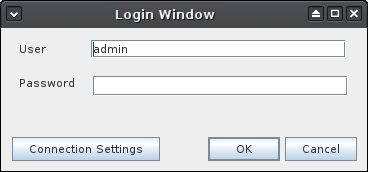
\includegraphics[width=0.5\linewidth]{img/auth_window.png}
		\caption{Authentication window}
		\label{fig:auth_window}
	\end{figure}
	The default connection settings should be enough if the server is running on the same computer as the client. If that's not the case, open the Connection Settings window (figure~\ref{fig:connection_settings}).
	\begin{figure}[h!]
		\centering
		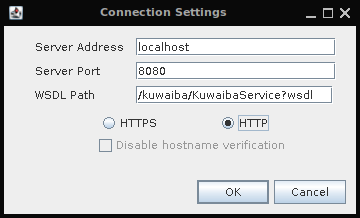
\includegraphics[width=0.5\linewidth]{img/connection_settings.png}
		\caption{Connection Settings window}
		\label{fig:connection_settings}
	\end{figure}
	\begin{itemize}
		\item \textbf{Server Address} Refers to the server IP address or canonical name.
		\item \textbf{Server Port} is the port Glassfish (the application server) is listening to.
		\item \textbf{WSDL Path} is the path within the application server the web service interface definition can be found. In most cases, this value shall remain unchanged.
		\item \textbf{Protocol} is the transport protocol to be used. By default is HTTP, but is highly recommended to request your administrator to setup a secure connection, otherwise your credentials will be transmitted in plain text over the network.
		\item \textbf{Disable host name verification} is disabled by default and applies only to HTTPS connections. If checked, the host name in the digital certificate does not have to have to match the host name you've typed in the "Server Address" field. This is useful if, for example, you are trying to connect to a server using its IP address, but the certificate was generated using its FQDN. You won't have to change this option in most cases, unless you are testing.
	\end{itemize}
	Except for the password, the last successful settings will be saved upon clicking OK.
	\begin{framed} {\large \textbf{Important}} \\
		If you are unsure if the server is reachable from your location, open a browser and type the address: \textbf{http://[server\_address]:[server\_port]/[wsdl\_location]}\\
		
		You should see a large XML document.
	\end{framed}
	\begin{framed} {\large \textbf{Troubleshooting}}
		\begin{itemize}
			\item For a \textbf{\textcolor{red}{Can't contact backend}} error, check the Administrator's Manual Troubleshooting section. This error is commonly associated with problems connecting to the database.
			\item If you get a \textbf{\textcolor{red}{Connection refused}} error, check the connection settings and verify that the server is reachable and there isn't a firewall blocking the traffic to it.
		\end{itemize}
	\end{framed} 
	Once you are logged in, you will see only the dashboard page and a toolbar (figure~\ref{fig:main_toolbar}).\\
	\begin{figure}[h!]
		\centering
		
\includegraphics[width=0.7\linewidth]{img/main_toolbar.png}
		\caption{Main toolbar}
		\label{fig:main_toolbar}
	\end{figure}
	
	The toolbar contains the most frequently used tools. Here is an overview of what you can do with them:
	\begin{table}[h!]
		\centering
		\begin{tabular}{cl}
			
\includegraphics[width=0.5cm]{img/icon_query_manager.png} & Search objects with the Query Manager\\
			\midrule
			
\includegraphics[width=0.5cm]{img/icon_refresh_component.png} & Refresh the current view\\
			\midrule
			
\includegraphics[width=0.5cm]{img/icon_refresh_cache.png} & Refresh local cache\\
			\midrule
			
\includegraphics[width=0.5cm]{img/icon_navigation_tree.png} & Main tree used to explore physical assets\\
			\midrule
			
\includegraphics[width=0.5cm]{img/icon_bookmarks.png} & Create and manage Favorite Folders and Favorites\\
			\midrule
			
\includegraphics[width=0.5cm]{img/icon_pools_manager.png} & Create and manage objects that don't have a place in the Navigation Tree\\
			\midrule
			
\includegraphics[width=0.5cm]{img/icon_relationship_explorer.png} & Explore an object's relationships\\
			\midrule
			
\includegraphics[width=0.5cm]{img/icon_special_children_explorer.png} & Explore the containment hierarchy used in models such as the Physical Layer model.\\
			\midrule
			
\includegraphics[width=0.5cm]{img/icon_topology_designer.png} & Freely design network topologies\\
			\midrule
			
\includegraphics[width=0.5cm]{img/icon_data_model_manager.png} & Manage the data model\\
			\midrule
			
\includegraphics[width=0.5cm]{img/icon_containment_manager.png} & Manage how objects can be created inside others\\
			\midrule
			
\includegraphics[width=0.5cm]{img/icon_list_type_manager.png} & Create new list types\\
			\midrule
			
\includegraphics[width=0.5cm]{img/icon_template_manager.png} & Create and manage templates\\
			\midrule
			
\includegraphics[width=0.5cm]{img/icon_user_manager.png} & Manage users and groups\\
			\midrule
			
\includegraphics[width=0.5cm]{img/icon_task_manager.png} & Create automation tasks (beta)\\
			\midrule
			
\includegraphics[width=0.5cm]{img/icon_reports.png} & Create and manage reports\\
			\midrule
			
\includegraphics[width=0.5cm]{img/icon_audit_trail.png} & Explore the application's log\\
			\midrule
			
\includegraphics[width=0.5cm]{img/icon_service_manager.png} & Manage customers, services and resources associated to them\\
			\midrule
			
\includegraphics[width=0.5cm]{img/icon_contract_manager.png} & Manage support contracts, SLAs and more. \\
			\midrule
			
\includegraphics[width=0.5cm]{img/icon_IPAM_manager.png} & Manage IPv4/IPv6 resources, such as IP addresses and subnets\\
			\midrule
			
\includegraphics[width=0.5cm]{img/icon_SDH_networks.png} & Manage Synchronous Digital Hierarchy resources\\
			\midrule
			
\includegraphics[width=0.5cm]{img/icon_MPLS_mudule.png} & Manage Multiprotocol Label Switching resources\\
			\midrule
			
\includegraphics[width=0.5cm]{img/icon_projects.png} & Manage projects, activities and resources associated to them\\
		\end{tabular}	
		\caption{Toolbar items}
		\label{tab:toolbar_icons}
	\end{table}
		
	\clearpage
	\section{Data Model Manager} \label{sec:data_model_manager}
		One of the key features of Kuwaiba is that it is completely object-oriented\footnote{Object-oriented Programming https://en.wikipedia.org/wiki/Object-oriented\_programming}. It means that every business (Router, City, Port) and application (users, types) element is represented by an \textbf{Object} in the application and these objects are in turn product of a reality abstraction called \textbf{Class}. Likewise, every attribute is a \textbf{Field} in a class. The set of classes, attributes and relationships between them is called \textbf{Data Model}. There's a default data model, but you can customize it depending on your needs by adding, removing and modifying classes. To achieve this, use the Data Model Manager module (figure~\ref{fig:data_model_manager}).
		\begin{figure}[h!]
			\centering
			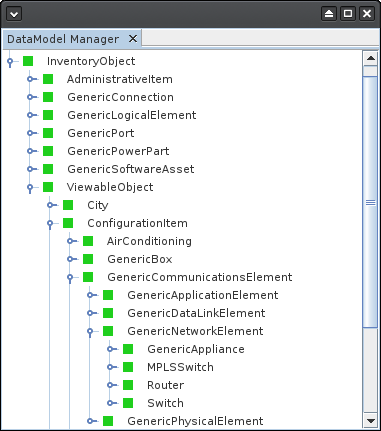
\includegraphics[width=0.4\linewidth]{img/data_model_manager.png}
			\caption{Data model tree section}
			\label{fig:data_model_manager}
		\end{figure}
		\begin{table}[h!]
			\centering
			\begin{tabular}{cp{10cm}}
				
\includegraphics[width=0.7cm]{img/icon_data_model_default_layout.png} & Resets the tree to its initial position (that is, with two root nodes: \textbf{GenericObjectList} and \textbf{InventoryObject}).\\
				\midrule
				
\includegraphics[width=0.7cm]{img/icon_data_model_class_hierarchy_view.png} & Opens a window with a graphical representation of the data model tree, easier to navigate.\\
				\midrule
				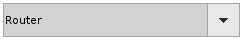
\includegraphics[width=5cm]{img/data_model_manager_search.png} & A shortcut to any class in the data model.\\
			\end{tabular}
			\caption{Data Model manager toolbar items}
			\label{tab:data_model_manager_toolbar_icons}
		\end{table}
		\subsection{Class Tree}
			The data model is represented as a tree because it's a hierarchical structure. Technically, it's a class hierarchy\footnote{Class Hierarchy https://en.wikipedia.org/wiki/Class\_hierarchy}. The top of the hierarchy (\textbf{InventoryObject}) is the most general type of element in the data model and its subclasses represent all the possible elements that will be treated as inventory assets. As you dig deeper into the tree, the classes become more and more specialized and each level inherits the attributes of the parent classes. This kind of structure has two purposes: First, it helps you to organize your classes based on what characteristics they have in common. Secondly, as you will see later in this manual, you can apply operations over top level classes, and they will be propagated to all subclasses. Another root of the data model tree is \textbf{GenericObjectList}, and its subclasses are all possible list types (see more details on the subject in the chapter \textbf{\nameref{sec:list_type_manager}}).\newline
			
			\begin{framed} {\large \textbf{Important}} \\
					The \textbf{Properties} window allows you to modify the attributes of a selected object in a tree, list or view. If not already open, it's available from the Windows $\rightarrow$ Properties menu item.
			\end{framed}
			The properties of a class can be edited by using the \textbf{Properties} window, selecting a class from the tree (see figure~\ref{fig:properties_class_node}). 
			\begin{figure}[h!]
				\centering
				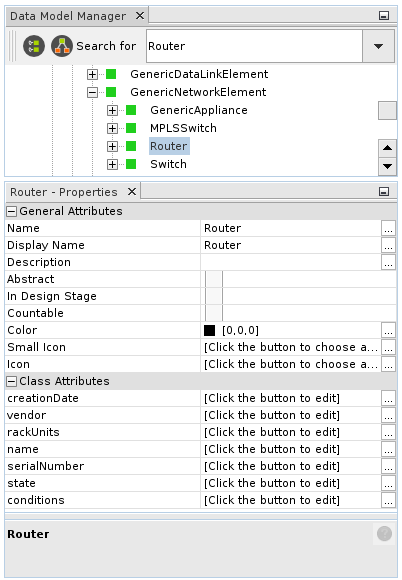
\includegraphics[width=0.5\linewidth]{img/data_model_manager_properties_class_node.png}
				\caption{Properties of class \textbf{Router}}
				\label{fig:properties_class_node}
			\end{figure}
			The  property  sheet  is  divided  in  two  sections: 
			\begin{itemize}
				\item \textbf{General:} Contains the intrinsic properties  of  the class: \textbf{name} (can contain only letters and numbers with no special characters  or  blank  spaces). The  \textbf{display name} of the class, that's how it  will be displayed everywhere else (useful  for  internationalization  purposes, for example) and can contain any kind of UTF-8 character. A \textbf{description} (useful  to  document  the  data  model). If  the class is \textbf{abstract} (abstract classes  cannot  be  instantiated, they're only used to give consistency to the  data  model). The attribute \textbf{countable} is not used currently, but it should be used to mark classes whose instances can have graphical representations, but  they're  not really  part  of  the  inventory,  such  as  \textbf{Slots}. \textbf{In Design Stage} is just a way to mark a class as part of an ongoing data model intervention, and thus, classes with that attribute set to true can not be instantiated. \textbf{Color} is the color of the default square icon used to display the object in a tree or view. This icon will be used as long as the \textbf{Small Icon} attribute is null. \textbf{Small Icon} is the icon that will be used in trees and its size can't exceed 16x16 pixels. \textbf{Icon} is the icon used in views, and has a maximum size of 32x32 pixels.
				\begin{framed} {\large \textbf{Important}}
					\begin{itemize}
						\item All user-created classes are set In Design Stage \textbf{\textcolor{green}{true}} by default. You won't be able to create objects from these classes until you set it to \textbf{\textcolor{blue}{false}}. It's just a precaution in case you are creating many classes at once and you want to test the changes before going to production.
						\item As a convention, all abstract classes have the prefix \textbf{Generic}. Note that a few core classes (like \textbf{InventoryObject} or \textbf{AdministrativeItem}) are abstract and are the exception to this rule. You, however, should try to follow this convention as much as possible. Unless you know what you are doing don't rename or delete core classes, mainly the abstract ones.
					\end{itemize}
				\end{framed}
				\item The second section  contains the class fields (attributes). In the  figure~\ref{fig:properties_class_node}, class Router  has six attributes: name, state, conditions, vendor, serialNumber and creationDate. Click the button next to the attribute name to customize it (see figure~\ref{fig:class_attribute_details}).
				\begin{figure}[h!]
					\centering
					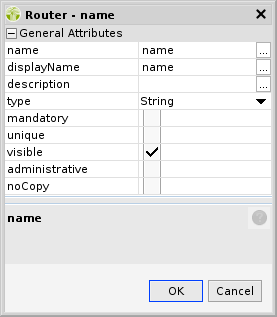
\includegraphics[width=0.4\linewidth]{img/data_model_manager_class_attribute_details.png}
					\caption{Properties of attribute \textbf{name} in class \textbf{Router}}
					\label{fig:class_attribute_details}
				\end{figure}
			\end{itemize}
			In this window, you can modify the attribute's name, display name, description, type  (the drop-down list will show you primitive types -String, Integer, Float, Long, etc- and all available non-abstract list types). When you change an attribute's type, all existing instances will be	modified to reflect the change, which means that the values of the modified attribute will be converted to the new type if possible (say, from Integers to Strings). If the conversion is not possible, the new value will be set to null.  You can also manage if the attribute is:
			\newline \textbf{mandatory}, selecting this option, every object of this class must have a value for this attribute. If you enable this option, and there are already created objects of this class without a non-null value for this attribute, you'll get an error.  
			\newline \textbf{unique}, if its marked, it means that the value of this attribute can not be repeated across all the  created objects from this class or its subclasses.  Before you can set a class attribute as unique, you must check if the value of this attribute in every created object from this class or its subclases is unique.
			\newline \textbf{visible}, this enables/disables the attribute's visibility, if is not marked the attribute will not be displayed in the property sheets of the objects created from this class.  
			\newline \textbf{administrative}, attributes marked as “Administrative” will be shown in a separate tab in the object's property sheet. Sometimes, there are  attributes that are used only for administrative purposes and might confuse the end user if mixed with the regular attributes. 
			\newline \textbf{noCopy}, you can choose what attributes shouldn't be transferred from one object to another in a copy operation.
			
			
			\begin{framed} {\large \textbf{Important}}
				\begin{itemize}
					\item You may lose information when changing an attribute's type. Make sure the conversion to the new type is possible before you do it.
					\item Although there's a Cancel button at the bottom of the window, it does not	really work. When you perform a change, it's saved immediately.
					\item If you add, remove or rename attributes, the changes will only be reflected in the properties sheets of the inventory objects that have previously open once you launch the "Update" option from the context menu of the node representing such object.
				\end{itemize}
			\end{framed}
			You can also create and delete classes and attributes by right-clicking a class node (see figure~\ref{fig:class_node_menu})
			\begin{figure}[h!]
				\centering
				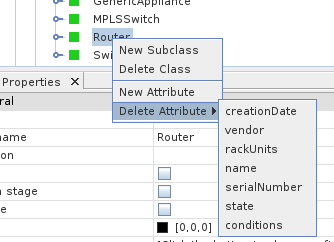
\includegraphics[width=0.7\linewidth]{img/class_node_menu.png}
				\caption{Class \textbf{Router} context menu}
				\label{fig:class_node_menu}
			\end{figure}
			New subclasses inherit the parent class attributes. Classes with instances or subclasses can not be deleted (this is  a  feature to avoid unintended loss of data). Also, attributes \textbf{creationDate} and \textbf{name} can not be deleted.
			\begin{framed} {\large \textbf{Important}}
				It's highly recommended \textbf{\textcolor{red}{NOT}} to rename abstract core classes, as some of them are used internally to support many features and renaming them may turn the system unstable.
			\end{framed}
	    \pagebreak
		\subsection{Class Hierarchy View}
			The data model can also be displayed on a canvas to improve the visualization and navigation. You can perform the same actions available in the standard tree view. To use it, click on the \textit{Class Hierarchy View} icon 
\includegraphics[width=0.7cm]{img/icon_data_model_class_hierarchy_view.png}, as seen in the Table~\ref{tab:data_model_manager_toolbar_icons}.
			\begin{table}[h!]
				\centering
				\begin{tabular}{cp{10cm}}
					
\includegraphics[width=0.7cm]{img/icon_expand_all.png} & Show all classes, without displaying the attributes\\
					\midrule
					
\includegraphics[width=0.7cm]{img/icon_collapse_all.png} & Collapse the tree, showing only the root class (\textbf{RootObject})\\
					\midrule
					
\includegraphics[width=0.7cm]{img/icon_expand_all_with_attributes.png} & Show all classes, displaying also their attributes\\
					\midrule
					
\includegraphics[width=0.7cm]{img/icon_organize.png} & If after expanding a class node it overlaps with another, use this button to organize again the tree\\
					\midrule
					
\includegraphics[width=0.7cm]{img/icon_export_as_image.png} & Export as Image Class Hierarchy\\
					\midrule
					
\includegraphics[width=0.7cm]{img/icon_export_as_xml.png} & Export as XML Class Hierarchy\\
					\midrule
					
\includegraphics[width=0.7cm]{img/icon_refresh_view.png} & Refresh Class Hierarchy view\\
					\midrule
					
\includegraphics[width=3cm]{img/data_model_manager_locate.png} & Locate a class in the tree\\
				\end{tabular}
				\caption{Class Hierarchy View toolbar icons}
				\label{tab:class_hierarchy_view_icons}
			\end{table}
			
			Each node of the tree represents a class and you can display/hide its attributes by expanding the node using the small triangle 
\includegraphics[width=0.5cm]{img/data_model_manager_triangle.png} at the top left corner of it. By default, and taking into account that the data model may have a considerable amount of classes, only the root class (\textbf{RootObject}) is displayed. You can either display the whole hierarchy by pressing the buttons 
\includegraphics[width=0.7cm]{img/icon_expand_all.png}/
\includegraphics[width=0.7cm]{img/icon_expand_all_with_attributes.png} or expanding one level at a time, using the right-click menu:
			\begin{figure}[h!]
				\centering
				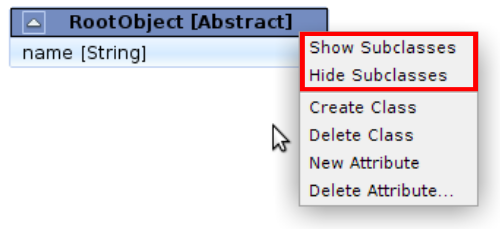
\includegraphics[width=0.5\linewidth]{img/data_model_manager_menu.png}
				\caption{Class node context menu}
				\label{fig:class_hierarchy_context_menu}
			\end{figure}
				
	\clearpage
	\section{Containment Manager} \label{sec:containment_manager}
	Another key concept in Kuwaiba is containment. It allows you to define what kind of objects can be created within others. For example, a \textbf{Country} can be inside a \textbf{Continent}, but can't be inside a \textbf{Rack}. A \textbf{Port} is usually within a \textbf{Board}, and not inside a \textbf{City}. These business rules can be defined using the Containment Manager.
	
	\subsection{Standard Containment Hierarchy} \label{sec:standard_containment_hierarchy}
	The main window is divided in two panels (see figure~\ref{fig:standard_containment_manager}, zoom in the image to see the details). The one on the left is a tree that holds all the classes plus the \textbf{Navigation Tree Root}. The children of the left-side tree node are the possible classes that can be contained. In the figure~\ref{fig:standard_containment_manager} there are five nodes expanded: \textbf{City}, that has one node inside: \textbf{Building}. That means that below a given city, you will only be able to add \textbf{Building} objects. Likewise, inside a \textbf{Continent} you can only create instances of \textbf{Country}, and inside those instances, only objects of class \textbf{City}. Under the root of the Navigation Tree, only instances of \textbf{Continent} are to be created. Finally, only \textbf{OpticalPorts} are supported under \textbf{DWDMBoards}. If for your operation Continents are not relevant, or if your routers do not have boards, but only ports, simplify the hierarchy as much as you want to meet your needs. To remove a possible children class, just right-click on it and select “Remove”, and instances from that class will no longer be available to be added under the parent class, though the objects already created will remain linked to the respective parent objects.
	
	\begin{figure}[h!]
		\centering
		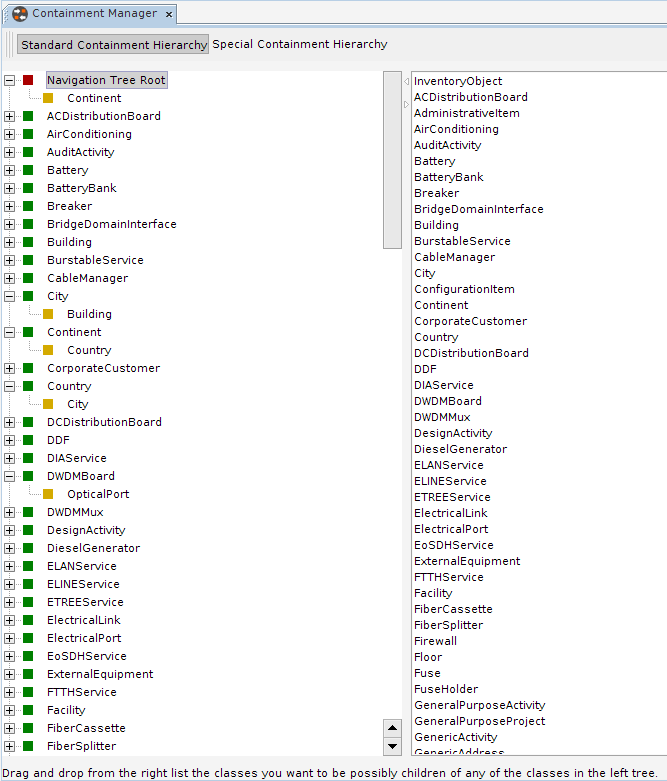
\includegraphics[width=0.7\linewidth]{img/standard_containment_manager.png}
		\caption{Standard Containment Manager main window. Zoom in the image if necessary}
		\label{fig:standard_containment_manager}
	\end{figure}
	
	\newpage
	
	\subsection{Special Containment Hierarchy} \label{sec:special_containment_hierarchy}
	The special containment hierarchy (see figure~\ref{fig:special_containment_manager}) is used to define containment rules for complex models. Most of the times you won't have to touch this, unless you are modeling new technologies and want to use containment relationships in your model that express a concept, rather than an one-to-one representation of the real world (e.g. you can use the special containment to represent how wavelengths/lambdas travel inside a fiber strand). Unlike the standard containment hierarchy, special children can only be explored using the \textbf{\nameref{sec:extra_explorers_children_explorer}}. The Physical Layer model is a good example of how this feature can be used: A cable inside a conduit connecting two buildings: in this scenario to configure the hierarchy for a wire container, drag links like (ElectricalLink, OpticalLink, PowerLink, RadioLink or for simply used the GenericPhysicalLink) from the right panel to the WireContainer class in the left panel, and in this way using the \textbf{\nameref{sec:extra_explorers_children_explorer}} you can create special children for a conduit. This is preconfigured in new databases so you don't have to worry about it.
	
	\begin{figure}[h!]
		\centering
		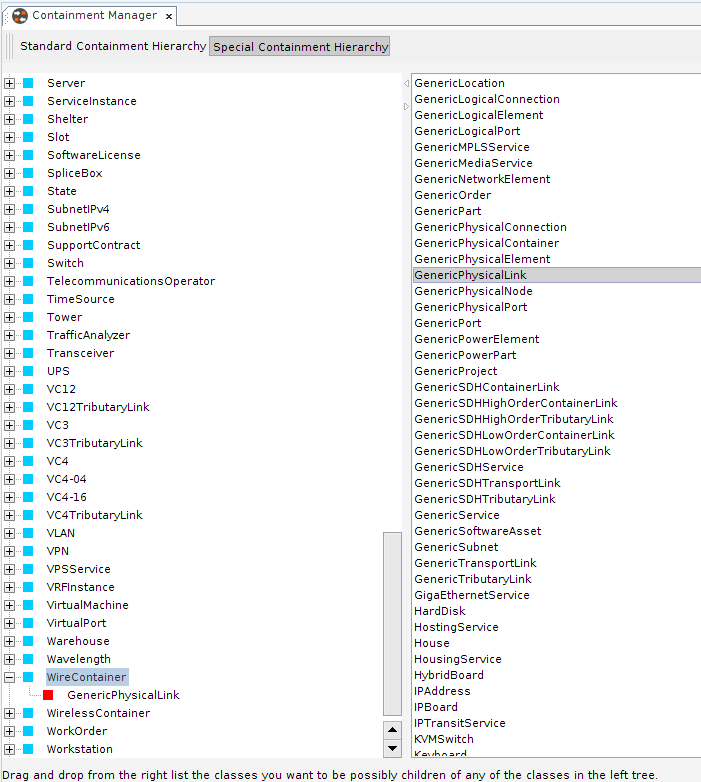
\includegraphics[width=0.8\linewidth]{img/special_containment_manager.png}
		\caption{Special Containment Manager main window. Zoom in the image if necessary}
		\label{fig:special_containment_manager}
	\end{figure}
	
	\begin{framed} {\large \textbf{Important}}
		\begin{itemize}
			\item To avoid adding one by one many classes to a parent, you can use the flexibility of the data model as a hierarchical structure. For example, a \textbf{Rack} may contain within many types of equipment (routers, DDFs, switches, battery banks, etc). Instead of adding each of these classes one by one, you can add a common super class and all of them will be added automatically. For this example a common super class for most of those classes could be \textbf{GenericCommunicationsElement}.
			\item To search for a particular class, just select any node in the desired side of the panel and type the first letters of the class name. If there are many occurrences of the term, jump from one to another using the F3 key.
			\item The changes are applied immediately, however, if you happen to not see them reflected, press the Refresh Cache button \includegraphics[width=0.5cm]{img/icon_refresh_cache.png} in the main toolbar (see table~\ref{tab:toolbar_icons}).
		\end{itemize}
	\end{framed}
			
	\clearpage
	\section{Navigation Tree} \label{sec:navigation_tree}
	This module presents in a tree fashion the physical objects of your inventory organized according to the standard containment hierarchy presented in the previous chapter (see \textbf{\nameref{sec:containment_manager}}).
	\begin{figure}[h!]
		\centering
		\includegraphics[width=0.4\linewidth]{img/navigation_tree.png}
		\caption{Navigation tree showing objects with default and user-defined icons}
		\label{fig:navigation_tree}
	\end{figure}
	Just like the \nameref{sec:data_model_manager}, the Properties window will display the attributes of the object selected in the Navigation Tree. These attributes match the visible attributes defined in the \textbf{\nameref{sec:containment_manager}}.
	\begin{figure}[h!]
		\centering
		\includegraphics[width=0.5\linewidth]{img/navigation_tree_properties.png}
		\caption{Properties of a selected \textbf{Rack} object}
		\label{fig:navigation_tree_properties}
	\end{figure}
	Every change is automatically committed to the database once you hit the Enter key. When editing dates, you need to select another attribute to commit the changes instead of pressing Enter. In the \textbf{\nameref{sec:containment_manager}} you can also configure what labels will be displayed instead of the actual names of the attributes and the help string in the lowest part of the window.\newline
	
	Every node has a set of actions, some will be active for all objects, some depend on the type of element that is selected. In the figure~\ref{fig:navigation_tree_context_menu} you can see the actions enabled for a \textbf{Rack} object. \\
	\begin{figure}[h!]
		\centering
		\includegraphics[width=0.7\linewidth]{img/navigation_tree_context_menu.png}
		\caption{Actions associated to the selected \textbf{Rack} object}
		\label{fig:navigation_tree_context_menu}
	\end{figure}
	\begin{itemize}
		\item \textbf{New:} The list of object types that can be contained for the selected element type according to the configured Containment Hierarchy. In this case, a \textbf{Rack} can contain \textbf{DDFs}, \textbf{ODFs}, \textbf{Routers}, etc.
		\item \textbf{New Multiple:} Creates a defined number of objects at once using a given name pattern (see \textbf{\nameref{app:AppendixA}} for details) figure~\ref{fig:new_multiple}.
			\begin{figure}[h!]
				\centering
				\includegraphics[width=0.5\linewidth]{img/new_multiple.png}
				\caption{Creation of a \textbf{Router} set}
				\label{fig:new_multiple}
			\end{figure}
		\item \textbf{New from template:} Creates an object (an possibly a complex containment structure under it) from a template defined previously. See more details in the chapter \nameref{sec:template_manager}.
		\item \textbf{Copy:} A plain copy operation.
		\item \textbf{Cut:} A plain cut operation.
		\item \textbf{Paste:} A plain paste operation. You can only paste objects where it is allowed according to the configured Standard Containment Hierarchy.
		\item \textbf{Update:} Updates the node information. Useful when a change has been made to the object from an external source (e.g. another user) or if you create a new list type affecting one of the attributes of the selected element. In this case, if you, for example, create an instance of \textbf{EquipmentVendor} (this will add a new entry to the \textbf{vendor} attribute list). Also use this action if you change the data model properties associated to the object class and want to see reflected in the property sheet (new attributes, renamed attributes, etc).
		\item \textbf{Edit:} Opens a Property Sheet to edit the attributes of the selected inventory object.
		\item \textbf{Delete:} Deletes the object. This will fail if the object has an incoming relationship, for example, a \textbf{Port} connected to a cable.
		\item \textbf{Reports:} The reports associated to the objects of this class. In this case, \textbf{Rack} has a report called \textbf{Rack Usage}. If no reports are associated, this entry will appear grayed out.
		\item \textbf{Relate To $\rightarrow$ Favorites Folder:} All inventory objects can be added to an existing Favorite Folder. See more details in the chapter \textbf{\nameref{sec:favorites}}.
		\item \textbf{Release From $\rightarrow$ Favorites Folder:} Removes the association between the selected object and a Favorites Folder.
		\item \textbf{Relate To $\rightarrow$ Service:} All inventory objects can be associated to an existing service. See more details in the chapter \textbf{\nameref{sec:service_manager}}.
		\item \textbf{Release From $\rightarrow$ Service:} Removes the association between the selected object and a service.
		\item \textbf{Show $\rightarrow$ Object View:} Opens the Object View to the selected object. See more details in the chapter \textbf{\nameref{sec:object_view_and_rack_view}}.
		\item \textbf{Show $\rightarrow$ Device Layout} Shows how the selected object looks in the real life, according to the layout designed using the \nameref{sec:template_manager}. Be aware that the selected object must be an instance of a subclass of \textbf{GenericCommunicationsElement} or \textbf{GenericFrame} and that it must have an attribute called \textbf{model} so this action is enabled.
		\item \textbf{Show $\rightarrow$ Rack View:} Opens the Rack view of the selected object. This action is only available for racks. See more details in the chapter \textbf{\nameref{sec:object_view_and_rack_view}}.
		
		\item \textbf{Relate To $\rightarrow$ Project:} All inventory objects can be a resource to an existing Project. See more details in the chapter \textbf{\nameref{sec:projects}}
		\item \textbf{Release From $\rightarrow$ Project:} Removes a selected object (resource) from a Project.
		\item \textbf{Relate To $\rightarrow$ Contract:} All inventory objects can be associated to an existing Contract. See more details in chapter \textbf{\nameref{sec:contract_manager}}
		\item \textbf{Release From $\rightarrow$ Contract:} Removes the association between an object and a contract.
		\item \textbf{Audit Trail:} This will display all the audit trail entries for the selected object, that is, all the changes made to it.
		\item \textbf{Diagnostics $\rightarrow$ Check Connections Integrity: } When you create a connection in the \nameref{sec:object_view_and_rack_view}, the parent of such connection is the object associated to the view. If you happen to move one of the endpoints of that connections to a parent outside that object, the connections might not show up again correctly in any view, so you must execute this action on the former parent, and the connections will be placed (and displayed) in the right place. It is expected that in future versions, this action expands its scope to diagnose some other possible integrity problems that could have been caused by custom task scripts or synchronization routines.
		\item \textbf{Create Physical Connection:} Creates a physical connection between \textbf{two} nodes selected in the Navigation Tree. This action will be disabled unless only two nodes are selected. See more details in the chapter \textbf{\nameref{sec:physical_connections}}.
		\item \textbf{Open an Explorer from Here:} Opens a Navigation tree whose root node will be the selected object. Useful when you want to explore an object with as many containment levels below.
		\item \textbf{Show More Information:} Shows the database id of the selected object. Useful for troubleshooting purposes. It will also show the object's complete containment structure. Note that the id can be used as search criteria in the \textbf{\nameref{sec:querying}}.
		\pagebreak
			\begin{figure}[h!]
				\centering
				\includegraphics[width=\linewidth]{img/action_show_object_id.png}
				\caption{Object id action on the selected \textbf{Rack} object}
				\label{fig:action_show_object_id}
			\end{figure}
	\end{itemize}
	\begin{framed} {\large \textbf{Important}}
		\begin{itemize}
			\item Remember that you can always open the Properties window by selecting the main menu option Windows $\rightarrow$ Properties.
			\item You can change the name of an object in-line by pressing F2 on a selected node (this trick will work on most modules).
		\end{itemize}
	\end{framed}
	\subsection{Relationships and Special Children Explorers} \label{sec:extra_explorers}
	Apart from the main navigation tree, there are also two explorers that are very useful to navigate through domain-specific models. Both explorers can be launched from the Tools $\rightarrow$ Navigation menu or using the icons \includegraphics[width=0.5cm]{img/icon_relationship_explorer.png} and \includegraphics[width=0.5cm]{img/icon_special_children_explorer.png}.

	\subsubsection{Relationship Explorer} \label{sec:extra_explorers_relationship_explorer}
		Allows to see the special relationships of the selected object. When an object makes part of a domain-specific model (SDH, Physical Connections, MPLS, Services, etc) there are special bounds to other objects called \textbf{relationships}. They have names documented on model-basis, and they can be seen using this explorer. In the figure~\ref{fig:navigation_tree_relationship_explorer}, it is depicted an \textbf{OpticalPort} with three relationships, one called \textbf{parent}, which all inventory objects has and is used to navigate upwards in the containment structure, the \textbf{endpointA} used in the Physical Connections model and it indicates that this port is the endpoint to a physical connection, probably a fiber optic. It also has a relationship called \textbf{uses}, which makes part of the Service management model. It indicates that the service called PDH Service-01 uses that port as a resource.
		
		\begin{figure}[h!]
			\centering
			\includegraphics[width=0.4\linewidth]{img/navigation_tree_relationship_explorer.png}
			\caption{Special relationships of the selected \textbf{OpticalPort} object}
			\label{fig:navigation_tree_relationship_explorer}
		\end{figure}
		
		The Relationships Explorer has a toolbar with a button that allows you to navigate through the special relationships using a canvas. To open the canvas (figure~\ref{fig:graphical_representation_relationships}) use the button \includegraphics[width=0.5cm]{img/icon_graphical_representation_relationships.png}.
						
		\begin{figure}[h!]
			\centering
			\includegraphics[width=0.8\linewidth]{img/graphical_representation_relationships.png}
			\caption{Special relationships canvas}
			\label{fig:graphical_representation_relationships}
		\end{figure}
			
		\begin{table}[h!]
			\centering
			\begin{tabular}{cl}
				\includegraphics[width=0.5cm]{img/icon_collapse_all.png} & Collapse the tree\\
				\midrule
				\includegraphics[width=0.5cm]{img/icon_export_as_image.png} & Export as image\\
				\midrule
				\includegraphics[width=0.5cm]{img/icon_reorganize_nodes.png} & If the nodes are overlapped, you can re-organize them using this button\\
    			\midrule
	 			\includegraphics[width=0.5cm]{img/icon_refresh_view.png} & Refresh the tree.\\
				\midrule
			\end{tabular}
			\caption{Toolbar options in the Special Relationships view}
			\label{tab:graphical_representation_relationships_toolbar_icons}
		\end{table}
			
		\subsubsection{Special Children Explorer} \label{sec:extra_explorers_children_explorer}							
		The special children are children as in the containment hierarchy concept, but used in domain-specific models, which gives them particular behavior depending on the situation (that is, they can't be handled as simple objects in the navigation tree because, for example, deleting them may require to perform tasks other than just removing the object from the database as they make part of a complex work flow). This is the case of the cables inside a conduit connecting two buildings. You can find more details about this scenario in the chapter \textbf{\nameref{sec:physical_connections}}.
						
		\begin{figure}[h!]
			\centering
			\includegraphics[width=0.7\linewidth]{img/navigation_tree_special_children_explorer.png}
			\caption{Fibers inside a container between two buildings}
			\label{fig:navigation_tree_special_children_explorer}
		\end{figure}
		
		Every node in the special children explorer has a set of actions. Some will be active for all objects, some depend on the type of element that is selected. In the figure~\ref{fig:navigation_tree_special_children_explorer} you can see the actions enabled for a WireContainer object. The actions are mostly the same as in the Navigation Tree with the following exceptions:
		
		\begin{itemize}
			\item \textbf{New Special:} The list of special object types that can be contained inside the selected element type as configured in the Special Containment Hierarchy.
			\item \textbf{New Special Multiple:} Creates a given number of special objects at once using a naming pattern see \textbf{\nameref{app:AppendixA}}
			\begin{figure}[h!]
				\centering
				\includegraphics[width=0.5\linewidth]{img/new_special_multiple.png}
				\caption{Creation of a \textbf{OpticalLink} set}
				\label{fig:new_special_multiple}
			\end{figure}			
			\item \textbf{New Special from template:} Creates a containment structure. See more details in the chapter \textbf{\nameref{sec:template_manager}}
		\end{itemize}
					
	\clearpage
	\section{Template Manager} \label{sec:template_manager}
	In many scenarios there are some containment structures that are created recurrently, like Building $\rightarrow$ Floor $\rightarrow$ Room $\rightarrow$ Rack, or ODF/DDFs with the same number of ports (12/24/36/48/72/96/144), or simply equipment with the same set of attributes, for example all the routers of a certain model: The vendor, number of rack units, slots, etc will be always the same. Creating them from scratch every time is a tedious task. For this reason, Kuwaiba provides a module that allows you to create templates of objects out of actual inventory elements. Go to Tools $\rightarrow$ Template Manager to open it.
	
	\begin{figure}[h!]
		\centering
		\includegraphics[width=0.4\linewidth]{img/template_manager_intro.png}
		\caption{Template Manager explorer}
		\label{fig:template_manager_intro}
	\end{figure}

	What you will see is a tree similar to that of the \ref{fig:data_model_manager}. The only difference is that no abstract or list type classes are listed. In the tree, locate the class which you want to create the template for, right click on the corresponding node and select \textit{New Template}.
	
	\begin{figure}[h!]
		\centering
		\includegraphics[width=0.3\linewidth]{img/template_manager_new_template.png}
		\caption{New Template}
		\label{fig:template_manager_new_template}
	\end{figure}
	
	Enter the name of the template and that's all. Choose a descriptive name, because that is the name you will see in the list of available templates for a particular class (e.g. "96-port ODF" or "Cisco ASR 1000")
	
	\begin{figure}[h!]
		\centering
		\includegraphics[width=0.6\linewidth]{img/template_manager_template_name.png}
		\caption{Template name}
		\label{fig:template_manager_name}
	\end{figure}
	
	Template elements properties can be edited the same way as the inventory objects. The values in the template (except for the creation date) will be copied onto the new objects created from them. The name of template objects for physical connections (links and containers) will be overriden with the one provided in the wizard.
	\newpage
	\begin{figure}[h!]
		\centering
		\includegraphics[width=0.6\linewidth]{img/template_manager_template_properties.png}
		\caption{Template element properties}
		\label{fig:template_manager_template_properties}
	\end{figure}
	
	You can also create templates from special objects. Note that the templates you create for classes \textit{GenericPhysicalContainer} and \textit{GenericPhysicalLink} will be used in the Physical Connections Wizard (see \textbf{\nameref{sec:physical_connections}}). The Figure \ref{fig:template_with_special_objects} shows the template for a Non-Armored Loose Tube Cable. 
	
	\begin{figure}[h!]
		\centering
		\includegraphics[width=0.6\linewidth]{img/template_with_special_objects.png}
		\caption{Template using special object}
		\label{fig:template_with_special_objects}
	\end{figure}
	
	Now you can create containment structures as complex as you want.\\
	
	\begin{figure}[h!]
		\centering
		\includegraphics[width=0.4\linewidth]{img/template_manager_template_containment.png}
		\caption{Template with a complex containment structure}
		\label{fig:template_manager_template_containment}
	\end{figure}
	Copy, paste and rename operations work as they do with normal inventory objects and you can use them to build your templates. Remember that you have to correctly configure the standard (see \ref{fig:standard_containment_manager}) and special (see \ref{fig:special_containment_manager}) containment hierarchy before creating templates.\\
	Now you can create objects from templates. Simply right-click on the parent object and select the \textbf{New from Template...} action.\\
	\begin{figure}[h!]
		\centering
		\includegraphics[width=0.6\linewidth]{img/template_manager_new_from_template.png}
		\caption{Creating a new object from a template}
		\label{fig:template_manager_new_from_template}
	\end{figure}
	
	\newpage
	Now select the desired template and select \textbf{Create Object}. Note that the window won't close automatically, so you can create more objects.
	\begin{figure}[h!]
		\centering
		\includegraphics[width=0.5\linewidth]{img/template_manager_select_template.png}
		\caption{Selecting a template}
		\label{fig:template_manager_select_template}
	\end{figure}

	\subsection{Layouts} \label{sec:layouts}
	In the template module the subclasses of  can have layout, this layout will be displayed in the rack view
	\begin{figure}[h!]
		\centering
		\includegraphics[width=0.5\linewidth]{img/template_manager_edit_layout.png}
		\caption{Edit a layout}
		\label{fig:template_manager_edit_layout}
	\end{figure}
	
	\subsection{Device Layout Editor} \label{sec:device_layout_editor}
	A layout is a set of basic shapes and custom shapes that represent the look of a device, generally for the case of devices that are located in a rack, this look belongs to the back, where the slots, modules and ports are shown, for these cases the layout is used to build the rack view (see \textbf{\nameref{sec:rack_view}}).
	\newpage
	
	To access in the device layout editor use the \textbf{\nameref{sec:template_manager}} selecting a template element and click Edit Layout \textbf{Figure~\ref{fig:device_layout_edit}}, if the attribute \textbf{model} is not fixed the action must be show disabled. To enable the Edit Layout action the attribute \textbf{model} must be created using the \textbf{\nameref{sec:data_model_manager}} the type of this attribute will be a list type, now create a list type item using \textbf{\nameref{sec:list_type_manager}} to set the model in the device and open the edit layout. \textbf{Figure~\ref{fig:device_layout_empty}}
		
	\begin{figure}[h!]
		\centering
		\includegraphics[width=0.9\linewidth]{img/device_layout_edit.png}
		\caption{Edit Device Layout}
		\label{fig:device_layout_edit}
	\end{figure}
		
	The first look of the device layout editor is an empty canvas \textbf{Figure~\ref{fig:device_layout_empty}} with a guide to draw devices that can be located in a rack like a Router, and the palette use to drag and drop shapes in the canvas to build the layout, also has a toolbar describe below.
	
	\begin{table}[h!]
		\centering
		\begin{tabular}[h!]{lp{10cm}}
			\includegraphics[width=0.5cm]{img/device_layout_save.png} & Save the Device Layout\\
			\midrule
			\includegraphics[width=0.5cm]{img/device_layout_delete.png} & Delete a saved Device Layout\\
			\midrule
			\includegraphics[width=0.5cm]{img/device_layout_clean.png} & Clean the Device Layout canvas\\
			\midrule
			\includegraphics[width=0.5cm]{img/device_layout_group.png} & Create a shape to group shapes\\
			\midrule
			\includegraphics[width=0.5cm]{img/device_layout_guide.png} & Show a guide to define the layout of a device which can be located in a rack\\
			\midrule
			\includegraphics[width=0.5cm]{img/device_layout_custom_shapes.png} & Show the Custom Shapes layout manager\\
			\midrule
			\includegraphics[width=0.5cm]{img/device_layout_show_palette.png} & Show the palette of shapes\\
			\midrule
		\end{tabular}
	\end{table}
		
	\begin{figure}[h!]
		\centering
		\includegraphics[width=0.9\linewidth]{img/device_layout_empty.png}
		\caption{Device Layout Editor}
		\label{fig:device_layout_empty}
	\end{figure}
	\newpage	
	
	The basic shapes and custom shapes that you drop in the canvas has a set of general properties and a set of unique properties \textbf{Figure~\ref{fig:device_layout_edited}} as is shown which allow to modify the shape. Also you can resize and move the shape in the canvas, and use the actions of copy and paste, and bring to front and back to fix the shape.
	
	\begin{figure}[h!]
		\centering
		\includegraphics[width=0.9\linewidth]{img/device_layout_edited.png}
		\caption{Editing Device Layout}
		\label{fig:device_layout_edited}
	\end{figure}
	
	If you see in the satellite view of the Device Layout Editor, there are two rectangles empty \textbf{Figure~\ref{fig:device_layout_edited}}, we call to this \textbf{slot} and inside can contain another device layouts. In the template element Cisco ASR 9001 has 2 slots the Slot-Module 0/0/0 and the Slot-Module 0/0/1, that slots are the two rectangles.
	
	The idea behind of slot is that you can replace layouts depending on the devices, for example the Slot-Module 0/0/0 has an A9K-MPA-20X1GE if you want render some layout this IPBoard must be has an attribute model assigned with a list type item, and a device layout edited \textbf{Figure~\ref{fig:device_layout_ipboard}}
	
	\begin{figure}[h!]
		\centering
		\includegraphics[width=0.99\linewidth]{img/device_layout_ipboard.png}
		\caption{Editing IPBoard Layout}
		\label{fig:device_layout_ipboard}
	\end{figure}
    \newpage
    
	When creating a design for a IPBoard like the A9K-MPA-20X1GE, it is likely that you need the name of the ports to be dynamic, and in this way make the design independent of the location of the IPBoard on a device. To solve this, the name of the shape can be a regular expression \textbf{Figure~\ref{fig:device_layout_port_naming}}, where the user can define his own expression using the notation of Java (java.util.regex) or use the predefined ones such as the \textbf{Cisco Port Naming}, in the case that does not require using a regular expression simply type a name.
	
	\begin{figure}[h!]
		\centering
		\includegraphics[width=0.99\linewidth]{img/device_layout_port_naming.png}
		\caption{Editing IPBoard Layout}
		\label{fig:device_layout_port_naming}
	\end{figure}
    \newpage
	
	Once defined the devices layout you can create a new object from template and use the action \textbf{Show $\rightarrow$ Device Layout} to see the layout. If the device no has a defined a device layout for the model then show a default layout \textbf{Figure~\ref{fig:device_layout_default}}.
	
	\begin{figure}[h!]
		\centering
		\includegraphics[width=0.99\linewidth]{img/device_layout_default.png}
		\caption{Render of Default Layout for Cisco ASR 9001 Ninth Av}
		\label{fig:device_layout_default}
	\end{figure}
	
	If the model has a layout assigned then render device layout created \textbf{Figure~\ref{fig:device_layout_render}}.
	
	\begin{figure}[h!]
		\centering
		\includegraphics[width=0.99\linewidth]{img/device_layout_show.png}
		\caption{Render of Cisco ASR 9001 Ninth Av}
		\label{fig:device_layout_render}
	\end{figure}
			
	\clearpage
	\section{List Type Manager} \label{sec:list_type_manager}
	Most of the attributes are primitive types (String, Integer, Booleans, etc), however, there are some more complex that are actually another object in the database. This is the case of attributes such as \textit{vendor}, which points to an object holding the information about the vendor of that equipment (support lines, account manager, etc) or \textit{state}, that refers to the current operational state of the equipment (Working, Not Working, Stored, etc) and the state itself is an object, because it may hold information about what are the next allowed states, for example. Many objects in the database will have the same \textit{vendor}, and many other will have the same \textit{state}. In short, list types are those kind of attributes that point to an element in a limited set of objects. In terms of relational databases, you can see it as a many-to-one kind of relationship. To manage the existing list types and its instances, use the \textbf{\nameref{sec:data_model_manager}} and the \textbf{\nameref{sec:list_type_manager}}. \newline
	
	To add new list types, add a subclass under GenericObjectList directly or any of its utility subclasses. List types are like any other class, you can customize them as needed.
	\begin{figure}[h!]
		\centering
		\includegraphics[width=0.5\linewidth]{img/list_type_own_type.png}
		\caption{Custom list type}
		\label{fig:list_type_own_type}
	\end{figure}
	 To create list type items, use the button \includegraphics[width=0.5cm]{img/icon_list_type_manager.png} or the menu option Tools $\rightarrow$ Administrative $\rightarrow$ List Type Manager. This module consists of a simple navigation tree similar to the one seen in the past chapter.
	 \begin{figure}[h!]
	 	\centering
	 	\includegraphics[width=0.3\linewidth]{img/list_type_list_type_items.png}
	 	\caption{Custom list type items}
	 	\label{fig:list_type_list_type_items}
	 \end{figure}
	 
	 By right-clicking and choosing \textit{New} on a selected list type, you can create new items. The details for every item can be edited using the standard Properties Window as seen in the past chapter. 
	 \newpage
	 \begin{framed} {\large \textbf{Important}}\\
	 	If the changes are not immediately reflected when editing an object, use the Refresh Cache button  \includegraphics[width=0.5cm]{img/icon_refresh_cache.png} and update the object (Right-click the object node and select the option \textit{Update}).
	 \end{framed}
	 
	 In the figure~\ref{fig:list_type_applied_types} you can see the properties of an object of class \textbf{Router} modified to have an attribute called \textit{myOwnAttribute} of type \textbf{MyOwnListType}.\newline
	 \begin{figure}[h!]
	 	\centering
	 	\includegraphics[width=0.4\linewidth]{img/list_type_applied_types.png}
	 	\caption{Object of class \textbf{Router} with a custom listy type attribute}
	 	\label{fig:list_type_applied_types}
	 \end{figure}
	 
	\clearpage
	\section{Query Manager} \label{sec:querying}
	\subsection{Graphical Query Editor} 
	The query editor lets you make a search with a graphical interface, based on nodes to represent the search criteria and connections to express the relationships. Once selected, by clicking on the icon \includegraphics[width=0.5cm]{img/icon_query_manager.png} you will get a blank canvas with a toolbar on top with the following elements:
	\begin{figure}[h!]
		\centering
		\includegraphics[width=1.1\linewidth]{img/query_tool_bar.png}
		\caption{Graphical query editor general tool bar}
		\label{fig:query_tool_bar}
	\end{figure}
	
	The toolbar contains the most frequently used tools. Here is an overview of what can you do with them:
	\begin{table}[h!]
		\centering
		\begin{tabular}{cl}
			\includegraphics[width=3cm]{img/icon_select_class_query.png} & Select the element class you want to search for. \\
			\midrule
			\includegraphics[width=0.5cm]{img/icon_open.png} & Open a previously saved query\\
			\midrule
			\includegraphics[width=0.5cm]{img/icon_save_view.png} & Save the current query. The queries are stored in the database using an XML format\\
			\midrule
			\includegraphics[width=0.5cm]{img/icon_delete_saved_view.png} & Deletes a saved query\\
			\midrule
			\includegraphics[width=0.5cm]{img/icon_clean_query.png} & Cleans the current query\\
			\midrule
			\includegraphics[width=0.5cm]{img/icon_edit_saved_query.png} & Edit details about the current query (name, description and owner)\\
			\midrule
			\includegraphics[width=0.5cm]{img/icon_reorganize_nodes.png} & Organize the nodes automatically\\
			\midrule
			\includegraphics[width=0.5cm]{img/icon_execute_query.png} & Executes the current query\\
			\midrule
			\includegraphics[width=2.2cm]{img/icon_logical_connector_query.png} & Logical connector used to chain the query predicates, by default AND\\
			\midrule
			\includegraphics[width=2.2cm]{img/icon_result_limit_query.png} & Max number of results per page, default 10; only integer values are allowed\\
		\end{tabular}	
		\caption{Query Toolbar items}
		\label{tab:query_toolbar_icons}
	\end{table}
	
	When you select a class from the drop-down box, a graphical representation of it will be placed on the canvas,
	\begin{figure}[h!]
		\centering
		\includegraphics[width=0.9\linewidth]{img/querying_node_added.png}
		\caption{Node added after selecting a element class}
		\label{fig:query_node_added}
	\end{figure}
	in the figure~\ref{fig:query_node_added} the class Router was selected, and the corresponding node is created. You can search for a wider range of elements if you select an abstract class (often called GenericSomething). In the example above it will search for all Routers in the database, but if you choose GenericPhysicalNode it will search for all physical nodes, that is, all objects that can be connected using a container (see Chapter \textbf{\nameref{sec:physical_connections}} for more information about containers). That includes: buildings, rooms, floors, towers, shelters and facilities. Note that the root class node is colored green.
	
	\newpage
	\begin{framed} {\large \textbf{Important}}
		\begin{itemize}
			\item If you want to see all objects in the database (at least all relevant to the inventory) search for \textbf{InventoryObject}, which is the root of all classes related to the inventory. To see the complete hierarchy see related chapter \textbf{\nameref{sec:data_model_manager}}
		\end{itemize}
	\end{framed}
	
	Back to the original example, if you just leave the router without modifications and execute the query \includegraphics[width=0.5cm]{img/icon_execute_query.png}, it will search for all routers available in the database and it will show only a column with the object's display name.				
	
	\begin{figure}[h!]
		\centering
		\includegraphics[width=0.9\linewidth]{img/query_results.png}
		\caption{Query results for all the routers}
		\label{fig:query_results}
	\end{figure}
	
	\newpage
	The figure~\ref{fig:query_results} is shown in a new tab and also has a tool bar with the following buttons:
	
	\begin{table}[h!]
		\centering
		\begin{tabular}{cl}
			\includegraphics[width=0.5cm]{img/query_result_export.png} & Export the results to popular formats like CSV, XML\\
			\midrule
			\includegraphics[width=0.5cm]{img/query_results_previous_page.png} & Previous page\\
			\midrule
			\includegraphics[width=0.5cm]{img/query_results_next_page.png} & Next page\\
			\midrule
			\includegraphics[width=0.5cm]{img/query_results_all_results.png} & Show all results\\
		\end{tabular}	
		\caption{Query results toolbar items}
		\label{tab:query_results_toolbar_icons}
	\end{table}
	
	Now, if we want to see more fields related to the  elements found, we should use the "field visibility icons". They're those eyes you can see along with the attributes names. By default none of them are selected, which means that no additional fields will be shown in the result list but the objects themselves. Think of them like the parts of a conventional SQL sentence that follows the SELECT clause: \textbf{SELECT creationDate, serialNumber FROM Router}. You can obtain a query like this pushing the toggle buttons with the eyes on it beside \textbf{serialNumber} and \textbf{creationDate} as you can see in the figure~\ref{fig:query_node_attributes_selected}
	
	\begin{figure}[h!]
		\centering
		\includegraphics[width=0.9\linewidth]{img/query_node_attributes_selected.png}
		\caption{creationDate and serialNumber to be shown in the result list}
		\label{fig:query_node_attributes_selected}
	\end{figure}
	
	When selected, the visibility icon turns into an eye crossed by a red line. If you don't want this attribute to be shown in the result list, press it again. This is what you will see when you execute the query:
	
	\begin{figure}[h!]
		\centering
		\includegraphics[width=0.6\linewidth]{img/query_results_attributes_selected.png}
		\caption{Result set showing some fields}
		\label{fig:query_results_attributes_selected}
	\end{figure}
	
	Now you may be wondering why the attributes \textbf{vendor}, \textbf{conditions} and \textbf{state} have their visibility icons disabled. That's because they're list type attributes (See \ref{sec:list_type_manager} for details about list type attributes).  Comparing again to SQL, these attributes are related to other \textit{tables} (other classes, actually). You have two ways to use these list type attributes as criteria: the first is just selecting the attribute's checkbox and choosing from a list the value that you'd like to use:
	\begin{figure}[h!]
		\centering
		\includegraphics[width=0.9\linewidth]{img/query_vendor_selected.png}
		\caption{Using a list type attribute as filter}
		\label{fig:query_vendor_selected}
	\end{figure}
	
	Or you can pick manually what fields belonging to the relationship must be included in the result set. To do this, you first have to toggle the simple class node filter (in our example labeled as \textbf{Vendor [Filter]}) to a detailed view. You can do that by right-clicking on the node's header and choosing the option \textbf{Toggle Simple/Detailed view}:
	\begin{figure}[h!]
		\centering
		\includegraphics[width=0.9\linewidth]{img/query_toggle_detail_view.png}
		\caption{Changing the detail level on a class filter}
		\label{fig:query_toggle_detail_view}
	\end{figure}
	
	The result is a node similar to the root one, but colored light orange
	\begin{figure}[h!]
		\centering
		\includegraphics[width=0.8\linewidth]{img/query_detail_view.png}
		\caption{Expanded class node filter}
		\label{fig:query_detail_view}
	\end{figure}
	
	You can toggle the node to the original compress view by right-clicking on node's header and choosing the option \textbf{Toggle Simple/Detailed view} again.
	
	\begin{framed} {\large \textbf{Example}}
		\begin{itemize}
			\item We want to search for all routers and we want to see the fields creation date, serial number, vendor and operational state. That would take:
			\\1. Enabling the visibility icon for the attribute \textbf{creationDate}
			\\2. Checking the checkbox in the attributes  \textbf{vendor} and state and expanding the resulting nodes (we'll talk about the checkbox later in this chapter)
			\\3. Enabling the visibility icon for the attribute  \textbf{name} in both newly spawned nodes.
		\end{itemize}
	\end{framed}
	
	\newpage
	Let's see the figure~\ref{fig:query_multiple_nodes}
	\begin{figure}[h!]
		\centering
		\includegraphics[width=0.8\linewidth]{img/query_multiple_nodes.png}
		\caption{Simple query showing three fields from different classes}
		\label{fig:query_multiple_nodes}
	\end{figure}
	
	Resulting in a set like this:
	\begin{figure}[h!]
		\centering
		\includegraphics[width=0.9\linewidth]{img/query_results_multiple_nodes.png}
		\caption{Simple query showing three fields from different classes}
		\label{fig:query_results_multiple_nodes}
	\end{figure}
	\begin{framed} {\large \textbf{Important}}\\
		The operational states and vendors were created using the List Manager (under OperationalState and Vendor, respectively) and their properties set in the Properties window.
	\end{framed}			
	
	The checkboxes are used to construct the query predicates. Every time you select one of them, a new node is spawned. If the attribute is a basic one (String, Integer, Float, Boolean or Date), you will get a node like one of these (otherwise you will get the class nodes seen above):
	\begin{figure}[h!]
		\centering
		\includegraphics[width=0.3\linewidth]{img/query_string_filter.png}
		\caption{Filter for String values}
		\label{fig:query_string_filter}
	\end{figure}
	\begin{figure}[h!]
		\centering
		\includegraphics[width=0.4\linewidth]{img/query_filter_numeric.png}
		\caption{Filter for Numeric values}
		\label{fig:query_filter_numeric}
	\end{figure}
	\begin{figure}[h!]
		\centering
		\includegraphics[width=0.3\linewidth]{img/query_date_filter.png}
		\caption{Filter for Date values}
		\label{fig:query_date_filter}
	\end{figure}
	\newpage
	\begin{framed} {\large \textbf{Example 2:}}
		\begin{itemize}
			\item We're going to search for Routers whose \textbf{name} contains the string \textit{AS} and the operational \textbf{state} is equal to \textit{Working} and have \textit{Cisco} as \textbf{vendor}. The fields to be shown must be \textbf{creationDate} and \textbf{operationalState}. Note that the result limit is set to 1 per page.
			The query would look like this:
		\end{itemize}
	\end{framed}
	
	\begin{figure}[h!]
		\centering
		\includegraphics[width=1.1\linewidth]{img/query_example_2.png}
		\caption{Complex query using an AND logical connector}
		\label{fig:query_example_2}
	\end{figure}
	
	The condition \textbf{Equal to} is case sensitive, while \textbf{like} is not.
	\begin{figure}[h!]
		\centering
		\includegraphics[width=1.1\linewidth]{img/query_example_2_results.png}
		\caption{Result set for the complex query}
		\label{fig:query_example_2_results}
	\end{figure}
	If you hit the “Next Page” button \includegraphics[width=0.5cm]{img/icon_next_page.png} you will get the second page of results if there is one and so on. The “Show all” button \includegraphics[width=0.5cm]{img/icon_retrieve_all.png} will retrieve the full list of results.
	\newpage
	\subsection{Exporting Results}
	Currently can export the results to plain text formats: CSV and XML. To export the results, press the Export icon \includegraphics[width=0.5cm]{img/icon_export.png}, which will open a window to choose the location of the output file and its format:
	\begin{figure}[h!]
		\centering
		\includegraphics[width=0.5\linewidth]{img/query_result_exportmenu.png}
		\caption{Results export options}
		\label{fig:query_result_exportmenu}
	\end{figure}
	
	\textbf{Export to} contains the file destination (once you choose a directory with the chosen file, a random name will be generated, but you can change it as you wish). Note that writing file the extension is not mandatory, since it will detect the type and append the extension before to save the file.  
	
	\textbf{Format} lets you choose the output format. The configure button \includegraphics[width=0.5cm]{img/icon_edit_saved_query.png} lets you set some particular options regarding to the selected format. Currently only CSV has advanced options:		
	\begin{figure}[h!]
		\centering
		\includegraphics[width=0.3\linewidth]{img/query_exports_settings.png}
		\caption{CSV filter settings}
		\label{fig:query_exports_settings}
	\end{figure}
	
	There you can choose the separator character between fields. The available options are: Comma(,), Tab (	), Space ( ), Pipe (|) and Tilde (~).
	
	Finally \textbf{Range} is used to specify whether whole results should be exported or only the current page.
	
	Note: The XML structure used to export the results can be checked in kuwaiba's wiki\footnote{Kuwaiba queries in XML format \detokenize{http://neotropic.co/kuwaiba/wiki/index.php?title=XML_Documents#To_Save_Queries}}.
	
	\subsection{Saving and restoring queries}
	The queries can be saved as public or private. It's probable that someone wants to execute the same query on a regular basis and if that's the case for many users, he/she would want to let other users use such query. After you design a query, you can save it and this small window will prompt for some basic information:
	\begin{figure}[h!]
		\centering
		\includegraphics[width=0.5\linewidth]{img/query_save_menu.png}
		\caption{Setting the query metadata before saving it}
		\label{fig:query_save_menu}
	\end{figure}
	
	\textit{Name} is the query name.
	\textit{Description} is the query description
	The last check box lets you make the current query public. By default, the query is private, so you don't pollute the list of available queries for the rest of the users. You can change these settings anytime using the configure button \includegraphics[width=0.5cm]{img/icon_edit_saved_query.png}.
	To open a query, just use the open button\includegraphics[width=0.5cm]{img/icon_open.png}, then you will be asked if you want to see only your queries or both your queries and the public ones:
	\textit{clicking on \textbf{No} will show you both private and public, clicking on \textbf{Yes} will list only those owned by you}
	\begin{figure}[h!]
		\centering
		\includegraphics[width=0.5\linewidth]{img/query_save_as_private.png}
		\caption{Dialog to choose what queries should be listed}
		\label{fig:query_save_as_private}
	\end{figure}
	
	Now you just have to select the one you need and you're done! 
	\begin{figure}[h!]
		\centering
		\includegraphics[width=0.5\linewidth]{img/query_saved_queries.png}
		\caption{list of available queries}
		\label{fig:query_saved_queries}
	\end{figure}
	
	\begin{figure}[h!]
		\centering
		\includegraphics[width=0.7\linewidth]{img/query_filter_value_not_saved.png}
		\caption{list of available queries}
		\label{fig:query_filter_value_not_saved}
	\end{figure}
	
	\begin{framed} {\large \textbf{Important}}\\
		Please note that when a query is saved the values used to filter won't be saved, since the filter nodes are used as open parameters. For example: in figure~\ref{fig:query_filter_value_not_saved}, the value \textit{Manchester} won't be saved anywhere. Just the structure and the condition (\textbf{like}, in this case). The blue box is a parameter. It's supposed that you will fill it with the value you need depending on what you're looking for.
		\\Note 1: Expanding a list type and not selecting anything from it has the same effect as selecting the value \textbf{None (null)} in the compact view of the filter.
		\\Note 2: Every time you run a query, a new window with the results will be opened, so don't forget to close those you don't need to save memory.
	\end{framed}
	
	\clearpage
	\section{Pools} \label{sec:pools_manager}
	This module enables you to create pools of objects. Pools are general purpose buckets where objects that can't be placed in the standard navigation tree are put. Most of them are logical or administrative elements such as VLANs or VPNs. You can see a pool like a bag where you put things you don't know where else to put. To use this module, click on the icon  \includegraphics[width=0.5cm]{img/icon_pools_manager.png} in the main toolbar or go to the menu item Tools/Pools. It will open a navigation tree similar to the one used to browse through the containment hierarchy. The first time it will be empty; you can add new pools by right-clicking the root new and selecting "New Pool", as show in the figure below.
	\begin{figure}[h!]
		\centering
		\includegraphics[width=0.5\linewidth]{img/pools_actions.png}
		\caption{Creating a new pool}
		\label{fig:pools_actions}
	\end{figure}
	
	The dialog box will prompt you for the newly created pool name, its description and the kind of objects  you want to store inside. If you choose, let's say, "Router", it will let you store only instances of Router. On the other hand, if you choose an abstract class (this is any starting with “Generic” or one of the core classes like InventoryObject or ViewableObject) you will be able to place instances of any subclasses of theirs. 
	\begin{figure}[h!]
		\centering
		\includegraphics[width=0.5\linewidth]{img/pools_create_new_pool.png}
		\caption{Pool creation dialog}
		\label{fig:pools_create_new_pool}
	\end{figure}
	
	\newpage
	Once it's created, you can edit the pool attributes \textit{name} and \textit{description} in the property sheet.
	\begin{figure}[h!]
		\centering
		\includegraphics[width=0.5\linewidth]{img/pools_pool_properties.png}
		\caption{Pool properties}
		\label{fig:pools_pool_properties}
	\end{figure}
	
	You can add children to it. By right-clicking on the corresponding node you can access to all actions associated to it. 
	\begin{figure}[h!]
		\centering
		\includegraphics[width=0.5\linewidth]{img/pools_pool_action.png}
		\caption{Pools Actions}
		\label{fig:pools_pool_action}
	\end{figure}
	
	From that moment on, it behaves exactly like the Navigation Tree and you may have multiple containment levels as shown in the figure below in the figure~\ref{fig:pools_pool_object_properties}.	
	\begin{figure}[h!]
		\centering
		\includegraphics[width=0.3\linewidth]{img/pools_pool_object_properties.png}
		\caption{Pools object properties}
		\label{fig:pools_pool_object_properties}
	\end{figure}
				
	\clearpage
	\section{Object View and Rack View} \label{sec:object_view_and_rack_view}
	\begin{figure}[h!]
		\centering
		\includegraphics[width=0.6\linewidth]{img/actions_object_and_rack_views.png}
		\caption{Show Object and Rack View actions in the Navigation Tree context menu}
		\label{fig:actions_object_and_rack_views}
	\end{figure}
	\subsection{Object View} \label{sec:default_view}
		A view is a graphical representation of what's inside an object. All instances (objects) of subclasses of \textbf{ViewableObject} have an Object View that displays the direct children of the selected node. Most objects, except logical and administrative assets and a few physical ones such as slots and ports are subclasses of \textbf{ViewableObject}. To access this view, select a node in the navigation tree right-click on it and click on the action Show Object View. You may open as many object views as you want (prior to version 1.5, you had only one Object View window that was updated everytime you selected an object).
		\begin{figure}[h!]
			\centering
			\includegraphics[width=0.9\linewidth]{img/default_view.png}
			\caption{Physical View of the selected \textbf{Country} object}
			\label{fig:default_view}
		\end{figure}
		
		In the Physical View, you can move and connect the nodes, add a background and export the view. It is particularly useful at Room and City levels, because it will allow you to see how the children elements are located geographically (e.g. buildings) or in an enclosed space (racks in a data center as seen in figure~\ref{fig:room_plan}).	
		
		\begin{figure}[h!]
			\centering
			\includegraphics[width=0.8\linewidth]{img/room_plan.png}
			\caption{Physical View of the selected \textbf{Room} object}
			\label{fig:room_plan}
		\end{figure}
		
		\newpage
		Figure~\ref{fig:default_view_toolbar} shows all general purpose tools available in this window.
		\begin{figure}[h!]
			\centering
			\includegraphics[width=0.6\linewidth]{img/default_view_toolbar.png}
			\caption{Physical View toolbar}
			\label{fig:default_view_toolbar}
		\end{figure}
		
		\begin{table}[h!]
			\centering
			\begin{tabular}[h!]{lp{10cm}}
				\includegraphics[width=0.5cm]{img/icon_save.png} & Save view\\
				\midrule
				\includegraphics[width=0.5cm]{img/icon_add_background.png} & Add a background image\\
				\midrule
				\includegraphics[width=0.5cm]{img/icon_remove_background.png} & Remove the background image\\
				\midrule
				\includegraphics[width=0.5cm]{img/icon_toggle_conn_labels.png} & Hide/show the labels next to the connections\\
				\midrule
				\includegraphics[width=0.5cm]{img/object_view_high_contrast.png} & Show high contrast node labels (useful when the background is dark)\\
				\midrule
				\includegraphics[width=0.5cm]{img/icon_select_tool.png} & Select/Move tool (selected by default)\\
				\midrule
				\includegraphics[width=0.5cm]{img/object_view_container.png} & Connect two nodes using a container (See \textbf{\nameref{sec:physical_connections}} for more details on how to use it)\\
				\midrule
				\includegraphics[width=0.5cm]{img/object_view_link.png} & Connect two ports using links (See \textbf{\nameref{sec:physical_connections}} for more details on how to use it)\\	
				\midrule
				\includegraphics[width=0.5cm]{img/icon_export.png} & Export to image file\\
				\midrule
				\includegraphics[width=0.5cm]{img/icon_refresh_view.png} & Refresh view\\			
			\end{tabular}
		\end{table}
		
		\clearpage
		\subsection{Rack View} \label{sec:rack_view}
		This view works only with objects of class \textbf{Rack} or its subclasses. It shows how the elements contained within the selected object are organized, based on their positions and number of rack units used. It can be launched by selecting the option \textit{Show Rack View} in the object's context menu.
		\begin{figure}[h!]
			\centering
			\includegraphics[width=0.6\linewidth]{img/show_rack_view.png}
			\caption{How to show the rack view}
			\label{fig:rack_view_combobox}
		\end{figure}
		
		For this view to be correctly built, three conditions must be met:
		\begin{itemize}
			\item The rack must have its \textbf{rackUnits} attribute set to a valid integer value. This attribute stores the total number rack units supported by the rack. Typical values are 20, 28, 34, 40 or 45.
			\begin{figure}[h!]
				\centering
				\includegraphics[width=0.6\linewidth]{img/error_rack_view_not_rackunits.png}
				\caption{Error displayed when the rack does not have a valid value of rack units}
				\label{fig:error_rack_view_not_rackunits}
			\end{figure}
			\item The attribute \textbf{rackUnitsNumberingDescending} must exist, if the rack unit sorting has not been set numbering ascending is assumed. This attribute tells the view to render the rack units in ascending order (if \textbf{false}) or descending order (if \textbf{true}).
			\begin{figure}
				\centering
				\includegraphics[width=0.4\linewidth]{img/rack_units_numbering_descending_attribute.png}
				\caption{Attribute correctly set in a Rack}
				\label{fig:rack_units_numbering_descending_attribute}
			\end{figure}
			\item The attributes \textbf{rackUnits} and \textbf{position} must exist and be set to valid values in the elements contained inside the rack. \textbf{rackUnits} in this case, makes reference to the number of rack units occupied by the contained element, while \textbf{position} is the start position of the contained element, 1-based, numbered from top to bottom. Your equipment vendor usually provides this value. If the value of rackUnits is 0, the element won't be dislayed in the view (useful for elements like grounding bars, for example).
			\begin{figure}[h!]
				\centering
				\includegraphics[width=0.4\linewidth]{img/rack_view_attributes_contained_element.png}
				\caption{Attributes correctly set in a DDF contained inside a rack}
				\label{fig:rack_view_attributes_contained_element}
			\end{figure}
		\end{itemize}
		\newpage
		\begin{framed} {\large \textbf{Important}}
			\begin{itemize}
				\item The attribute name \textbf{rackUnitsNumberingDescending} is case-sensitive and must be Boolean.
				\item The attribute names (\textbf{rackUnits}, \textbf{position}) are case sensitive and must be integers.
				\item Some elements you want to create inside a rack \textbf{might not} have those attributes by default, so you will need to create them using the \nameref{sec:data_model_manager}.			
			\end{itemize}
		\end{framed}
		\newpage		
		If all values are correct, the view should look like this:
		\begin{figure}[h!]
			\centering
			\includegraphics[width=0.85\linewidth]{img/rack_view_sample_view.png}
			\caption{Sample rack view}
			\label{fig:rack_view_sample_view}
		\end{figure}

		In the Rack View you have a toolbar to export the view or refresh the last change in the view.
		
		\begin{figure}[h!]
			\centering
			\includegraphics[width=0.3\linewidth]{img/rack_view_toolbar.png}
			\caption{Rack View Toolbar}
			\label{fig:rack_view_toolbar}
		\end{figure}
		
		\begin{table}[h!]
			\centering
			\begin{tabular}[h!]{lp{10cm}}
				\includegraphics[width=0.5cm]{img/rack_view_export.png} & Export to image file\\
				\midrule
				\includegraphics[width=0.5cm]{img/rack_view_refresh.png} & Refresh Rack View\\
				\midrule
				\includegraphics[width=0.5cm]{img/rack_view_select.png} & Select a device\\
				\midrule
				\includegraphics[width=0.5cm]{img/rack_view_connect_ports.png} & Connects ports\\
				\midrule
				\includegraphics[width=0.5cm]{img/rack_view_table.png} & Show a list of connections in the selected rack\\
				\midrule
				\includegraphics[width=0.5cm]{img/rack_view_show_connections.png} & Show the device layouts and connections\\
				\midrule
			\end{tabular}
		\end{table}
		
		To see the connections in the rack click the button \includegraphics[width=0.7cm]{img/rack_view_show_connections.png} and a rack view is rendered using the devices layout or default layouts \textbf{Figure~\ref{fig:rack_view_connections}} (for more information about device layout see \textbf{\nameref{sec:device_layout_editor}})
		
		\begin{figure}[h!]
			\centering
			\includegraphics[width=0.95\linewidth]{img/rack_view_connections.png}
			\caption{Show Connections in Rack}
			\label{fig:rack_view_connections}
		\end{figure}
		
	\clearpage
	\section{Physical Connections} \label{sec:physical_connections}
		The Physical Connections toolkit is tightly integrated to the Physical View module. With Kuwaiba you can create physical layer connections using cables, fiber optics or radio links very easily, navigate through the connections and inspect the resources in use.\newline
		
		Before presenting the tools provided by the application, let's first clarify and introduce some concepts. This module deals solely with L1 topologies. It's only about cables, ports, etc. The data model provides four types of entities to represent physical layer elements:
		\begin{itemize}
			\item \textbf{Links:} These are all physical connections that connect two ports. In the current data model, there are three	types of connections: \textbf{ElectricalLink} (for electrical connections like coaxial, twisted
			pairs and the like), \textbf{OpticalLink} (for fiber optics), \textbf{RadioLink} (for radio links -Microwave links, mostly-) and \textbf{PowerLink} (for electrical power connections AC/DC). You can create new types by adding subclasses to the abstract class \textit{GenericPhysicalLink}
			\item \textbf{Containers:} All objects that can be used to contain, wrap and protect links (understanding \textit{Link} as defined above). There are two types of containers: \textbf{WireContainer} (used to contain all kind of cables -wires and fibers-, like pipes, conduits, ditches, etc) and \textbf{WirelessContainer} (used to contain radio channels or carriers). You can create new types by adding subclasses to the abstract class \textit{GenericPhysicalContainer}.
			\item \textbf{Nodes:} These objects are endpoints to \textit{Containers}. In the default data model you will find classes like: \textbf{Tower}, \textbf{Warehouse}, \textbf{Facility}, \textbf{Shelter}, \textbf{Building}, \textbf{Floor} and \textbf{Room}, but in general, any inventory object can be a \textit{Node}. In versions prior to 1.5, only subclasses of \textbf{GenericPhysicalNode} could be nodes.
			\textbf{Endpoints:} These objects are endpoints to \textit{Links}. In practice, they're always some kind of \textbf{Port} (in the data model context, this means all subclasses of \textbf{GenericPort}).
		\end{itemize}
		In summary, you can only connect \textit{Nodes} using \textit{Containers} and \textit{Endpoints} using \textit{Links}. To create new connections, open the Object View of an element and try to connect the desired nodes. For example, if you want to connect two buildings, select the city which is the parent for both. Likewise, if you want to connect a router to an ODF, you probably will have to select the room or the rack where they are located. In short, select the nearest common parent between the two elements you want to connect. Alternatively, you can just select two objects in the \ref{sec:navigation_tree} and execute the action \textit{Create Physical Connection}.
		
		Let's put together all these concepts with some examples. 
		\subsection{Example 1} \label{sec:physical_connections_example_1}
			In this example, we will create a direct connection between two routers in the same room, but in different racks using a CAT-5 patch as shown in the figure~\ref{fig:l1_example_1}.\newline
			\begin{figure}[h!]
				\centering
				\includegraphics[width=0.5\linewidth]{img/l1_example_1.png}
				\caption{Connection diagram for example 1}
				\label{fig:l1_example_1}
			\end{figure}
			
			Let's consider the layout in figure~\ref{fig:l1_example_1_layout}
			\begin{figure}[h!]
				\centering
				\includegraphics[width=0.3\linewidth]{img/l1_example_1_layout.png}
				\caption{Containment layout for example 1}
				\label{fig:l1_example_1_layout}
			\end{figure}
			\begin{enumerate}
				\item Select the nearest common parent in the navigation tree (in this case the \textbf{Room} called Control Center), and using the select tool, change the default position of the nodes
				\begin{figure}[h!]
					\centering
					\includegraphics[width=0.8\linewidth]{img/l1_example_1_initial_view.png}
					\caption{Racks in the room}
					\label{fig:l1_example_1_initial_view}
				\end{figure}
				\item Using the \textbf{\nameref{sec:list_type_manager}}, create a list type called \textit{CAT-5} under \textbf{ElectricalLinkType}. Following a similar procedure, you can create the different types of electrical connections depending on your network (POTS, coaxial, etc). We will use this later.
				\label{item:connection_type}
				\newpage
				\begin{figure}[h!]
					\centering
					\includegraphics[width=0.4\linewidth]{img/l1_example_1_electrical_link_type.png}
					\caption{Creating the link type}
					\label{fig:l1_example_1_electrical_link_type}
				\end{figure}
				\item Activating the connection tool, click on one node and hold, dragging the mouse until you reach the second node. Make sure you also select the button to link connections \includegraphics[width=0.5cm]{img/object_view_link.png}.
				\begin{figure}[h!]
					\centering
					\includegraphics[width=0.8\linewidth]{img/l1_example_1_new_connection.png}
					\caption{Creating the connection}
					\label{fig:l1_example_1_new_connection}
				\end{figure}
				\begin{figure}[h!]
					\centering
					\includegraphics[width=0.7\linewidth]{img/actions_create_connection_link.png}
					\caption{Creating a connection using the node action}
					\label{fig:actions_create_connection_link}
				\end{figure}
				\item This will open a wizard where you have to fill in the basic information about the connection: its name and class.
				\begin{figure}[h!]
					\centering
					\includegraphics[width=0.8\linewidth]{img/l1_example_1_link_wizard.png}
					\caption{Connection wizard, step 1}
					\label{fig:l1_example_1_new_link_wizard}
				\end{figure}
								
				\item In the next step of the wizard, you should select the endpoints of the connection (the end ports)
				\begin{figure}[h!]
					\centering
					\includegraphics[width=0.8\linewidth]{img/l1_example_1_endpoints.png}
					\caption{Connection wizard, step 2}
					\label{fig:l1_example_1_endpoints}
				\end{figure}
			\end{enumerate}
			
			And that's it. Double-clicking on the connection will add a control point to it. You can add as many as you want, and control its route. The Properties window will get updated accordingly if you select the link or a node.
			\begin{figure}[h!]
				\centering
				\includegraphics[width=0.6\linewidth]{img/l1_example_1_final.png}
				\caption{Final result}
				\label{fig:l1_example_1_final}
			\end{figure}
			\begin{framed} {\large \textbf{Important}}\\
				Don't forget to save the view using the icon \includegraphics[width=0.5cm]{img/icon_save.png} in the toolbar, so your positioning changes are stored.
			\end{framed}
			\clearpage	
			\subsubsection{Moving Links in and out of containers} \label{sec:move_physical_links}
				It is possible to move created links into a container, to move links into containers select the link or the links (using ctrl + click to select multiple links), then make right click in one of the links you want to move, this action will show you a new window to select one of the existing wire containers between de two end points of the selected links.
				\begin{figure}[h!]
					\centering
					\includegraphics[width=0.6\linewidth]{img/l1_selected_links_to_move_into_container.png}
					\caption{Selection of links to move into container}
					\label{fig:l1_selected_links_to_move_into_container}
				\end{figure}	

				\begin{figure}[h!]
					\centering
					\includegraphics[width=0.6\linewidth]{img/l1_list_of_existing_containers.png}
					\caption{Possible containers to move the selected links in}
					\label{fig:l1_list_of_existing_containers}
				\end{figure}	
	            \clearpage	
				It is also possible move links out of a wire container, make right click in wire container, this action will show you a new window to select the link(s) inside the wire container, selected the link or the links(using ctrl + click to select multiple links).
			
				\begin{figure}[h!]
					\centering
					\includegraphics[width=0.6\linewidth]{img/l1_selected_container_to_move_links_out.png}
					\caption{Selected wire container to move links out}
					\label{fig:l1_selected_container_to_move_links_out}
				\end{figure}	
			
				\begin{figure}[h!]
					\centering
					\includegraphics[width=0.6\linewidth]{img/l1_list_of_links_to_move.png}
					\caption{List of links to to move out of the wire container}
					\label{fig:l1_list_of_links_to_move}
				\end{figure}
	
		\subsection{Example 2}	
			The second example is more complex. We will connect two buildings with a conduit that contains fibers. In each building there's a router and an ODF. One of the fiber pairs connecting the buildings will be linking the two ODFs, and then, from the ODF, we'll patch our way to the routers.
			\begin{figure}[h!]
				\centering
				\includegraphics[width=0.8\linewidth]{img/l1_example_2.png}
				\caption{Connection diagram for example 2}
				\label{fig:l1_example_2}
			\end{figure}
			\newpage
			We will use a similar containment layout for this example, just adding a couple ODFs.
			\begin{figure}[h!]
				\centering
				\includegraphics[width=0.4\linewidth]{img/l1_example_2_layout.png}
				\caption{Containment layout for example 2}
				\label{fig:l1_example_2_layout}
			\end{figure}
			
			\begin{enumerate}
					\item First, we must make the initial arrangements. In this case, we will use a Google maps image as background for the city (the nearest common parent) and locate the buildings. We also select the connection tool and the connections to container tool \includegraphics[width=0.5cm]{img/object_view_container.png}.
					\begin{figure}[h!]
						\centering
						\includegraphics[width=\linewidth]{img/l1_example_2_initial_view.png}
						\caption{Buildings in the city}
						\label{fig:l1_example_2_initial_view}
					\end{figure}
					\begin{figure}[h!]
						\centering
						\includegraphics[width=0.7\linewidth]{img/actions_create_connection_container.png}
						\caption{Creating a connection using the node action}
						\label{fig:actions_create_connection_container}
					\end{figure}
					\newpage
					\item Since this time we are creating a \textbf{WireContainer}, the list type for it must be created under \textbf{WireContainerType}. Using the \nameref{sec:list_type_manager}, add this entry:
					\begin{figure}[h!]
						\centering
						\includegraphics[width=0.2\linewidth]{img/l1_example_1_wire_container_type.png}
						\caption{reating a connection type}
						\label{fig:l1_example_1_wire_container_type}
					\end{figure}
					\item Just like we did in the past example, let's start the connection wizard, we fill in the basic fields name of connection and container class in this case we use a \textbf{WireContainer}.
					\begin{figure}[h!]
						\centering
						\includegraphics[width=0.8\linewidth]{img/object_view_wizard_1.png}
						\caption{Connection wizard, step 1}
						\label{fig:l1_example_2_wizard_1}
					\end{figure}			
					\item In the second step just like we did in the past example, but this time the endpoints will be the buildings instead of the ports (remember that we are creating a container here).
					\begin{figure}[h!]
						\centering
						\includegraphics[width=0.8\linewidth]{img/l1_example_2_endpoints.png}
						\caption{Connection wizard, step 2}
						\label{fig:l1_example_2_endpoints}
					\end{figure}			
					\item Using the Select tool, modify the route of the connection. Now the container has been created successfully.
					\begin{figure}[h!]
						\centering
						\includegraphics[width=\linewidth]{img/l1_example_2_final.png}
						\caption{Final result}
						\label{fig:l1_example_2_final}
					\end{figure}
					\item Once the container has been created, you can now connect/disconnect the links or containers inside the newly created connection. In this example, we will connect a fiber strand (OpticalLink) to each side's ODF back port (note the naming used for the ODF ports in the figure~\ref{fig:l1_example_2_layout}). To start a wizard to perform this operation, right-click on the container and select the option \textit{Connect links...}
					\begin{figure}[h!]
						\centering
						\includegraphics[width=0.3\linewidth]{img/l1_example_2_container_context_menu.png}
						\caption{Container's contextual menu}
						\label{fig:l1_example_2_container_context_menu}
					\end{figure}
					\item This opens a window divided in three panels. The side panels let you choose what ports you want to connect to the fibers in the container. In this example, we will connect the first pair to the ports labeled as \textit{Back} in the ODFs. You can select multiple ports and fibers and connect them at the same time (use the SHIFT key for multiple selection). Note that it's not necessary to connect both sides. Push the \textit{Connect} button on the lower part of the central panel to finish the procedure.
					\begin{figure}[h!]
						\centering
						\includegraphics[width=0.9\linewidth]{img/l1_example_2_add_links.png}
						\caption{Adding links in the crated container}
						\label{fig:l1_example_2_add_links}
					\end{figure}
					\begin{figure}[h!]
						\centering
						\includegraphics[width=0.9\linewidth]{img/l1_example_2_connect_links.png}
						\caption{Connecting links}
						\label{fig:l1_example_2_connect_links}
					\end{figure}
					\begin{framed} {\large \textbf{Important}}
						\begin{itemize}
							\item In optical connections, Rx and Tx ports are treated as a single port and a pair of strands, is actually represented as a single \textbf{OpticalLink}.							
						\end{itemize}
					\end{framed}
					It's possible to explore the contents of a container and see to what fiber the ports are connected by using the explorers in the menu Tools $\rightarrow$ Navigation. In the figure~\ref{fig:l1_example_2_links_in_container} you will see the Special Children explorer when the container is selected in the view. In the figure~\ref{fig:l1_example_2_container_relationships}, the relationship explorer shows the connections of one of the ports in the ODF when selected in the \nameref{sec:navigation_tree}.
					\begin{figure}
						\centering
						\includegraphics[width=0.3\linewidth]{img/l1_example_2_links_in_container.png}
						\caption{Exploring the container's contents}
						\label{fig:l1_example_2_links_in_container}
					\end{figure}
					\begin{figure}
						\centering
						\includegraphics[width=0.4\linewidth]{img/l1_example_2_container_relationships.png}
						\caption{Exploring the container's relationships}
						\label{fig:l1_example_2_container_relationships}
					\end{figure}
					\item Now we will create an optical patch in each building between the routers and the 1-Front ports of their respective ODFs in a similar way we did in the \textbf{\nameref{sec:physical_connections_example_1}}.
					\begin{figure}[h!]
						\centering
						\includegraphics[width=0.5\linewidth]{img/l1_example_2_patch_a.png}\\
						\includegraphics[width=0.5\linewidth]{img/l1_example_2_patch_b.png}
						\caption{Optical patches between routers and ODFs}
						\label{fig:l1_example_2_patches}
					\end{figure}
					\begin{framed} {\large \textbf{Important}}\\
						\begin{itemize}
							\item 							Use an \textbf{OpticalLink} instead of an \textbf{ElectricalLink} if the connection represents a fiber strand.
							\item The color of the connections (logical and physical) is taken from the color assigned to the class in the \nameref{sec:data_model_manager}.
						\end{itemize}
						
					\end{framed}
					\item There's still one last step: The ports 1-Front and 1-Back in each ODF are not yet bridged. To do this, we just have to right-click any of the two ports on each ODF and select the option \textit{Connect Mirror Port...}. A mirror port is basically a direct connection between two ports. A cable is a separate object in Kuwaiba, a mirror connection is not even an object, it is just a relationship between a port an another with the same parent (that is, a sibling). You can see it as a backplane connection.
					To create multiple mirror ports see more details in \textbf{\nameref{app:multiple-mirror-ports}}
					\begin{figure}[h!]
						\centering
						\includegraphics[width=0.7\linewidth]{img/l1_example_2_mirror_connection_menu.png}
						\caption{Mirror connection menu}
						\label{fig:l1_example_2_mirror_connection_menu}
					\end{figure}
					\newpage
					This will open a window where you can select what port you want to be mirror of the selected one. Since 1-Front ports only have one sibling (1-Back), that's the only option available.
					\begin{figure}[h!]
						\centering
						\includegraphics[width=0.5\linewidth]{img/l1_example_2_mirror_connection_details.png}
						\caption{Mirror connection details}
						\label{fig:l1_example_2_mirror_connection_details}
					\end{figure}
					
					Once the port is mirrored, you can see a new relationship in the relationship explorer when selecting any of the ODF ports in the \textbf{\nameref{sec:navigation_tree}}.
					\begin{figure}[h!]
						\centering
						\includegraphics[width=0.4\linewidth]{img/l1_example_2_mirror_connection_relationships.png}
						\caption{Mirror connection relationship}
						\label{fig:l1_example_2_mirror_connection_relationships}
					\end{figure}
					
					To release a mirror port, select the option from the context port's context menu.
					\begin{figure}[h!]
						\centering
						\includegraphics[width=0.5\linewidth]{img/l1_example_2_mirror_connection_release.png}
						\caption{Release mirror connection menu option}
						\label{fig:l1_example_2_mirror_connection_release}
					\end{figure}
			\end{enumerate}
			
			A nice feature in Kuwaiba is the ability to see the path of a physical connection as long as there's continuity. In our example, there is continuity between the port in the router A (RTR-DMT-003) and the port in the Router B (RTR-DMT-004), that is, there are no active elements in between. To see the trace, right-click on any of the ports involved in the connection and select the option \textit{Show physical path}.
			\begin{figure}[h!]
				\centering
				\includegraphics[width=0.3\linewidth]{img/l1_example_2_physical_path_menu.png}
				\caption{Physical path menu option}
				\label{fig:l1_example_2_physical_path_menu}
			\end{figure}
			The figure~\ref{fig:l1_example_2_physical_path_list} show the physical path between Router A's port and Router B's port. The port in red is where the trace begins.
			\begin{figure}[h!]
				\centering
				\includegraphics[width=0.4\linewidth]{img/l1_example_2_physical_path_list.png}
				\caption{Physical path details}
				\label{fig:l1_example_2_physical_path_list}
			\end{figure}
			
			And pressing the button \includegraphics[width=0.5cm]{img/icon_physical_path_graphical.png} you will get a graphical representation, easier to understand.
			\begin{figure}[h!]
				\centering
				\includegraphics[width=1.1\linewidth]{img/l1_example_2_physical_path_view.png}
				\caption{Physical path graphical representation}
				\label{fig:l1_example_2_physical_path_view}
			\end{figure}
			The Properties window will be updated as you select any of the blocks. This view can also be updated.
			
	\clearpage
	\section{Audit Trail} \label{sec:audit_trail}
	Kuwaiba is capable of tracking the changes performed by the users in the database for audit purposes. These changes can be made to inventory objects (equipment, locations, etc) or application objects (pools, tasks, user properties). There are two types of events that are logged: \textbf{General events}, that is, those that are not related to any object in particular, like new logins or creation of application objects. \textbf{Object-related events}, like property changes or move operations.
	\begin{figure}[h!]
		\centering
		\includegraphics[width=\linewidth]{img/audit_trail_general_events.png}
		\caption{General events window}
		\label{fig:audit_trail_general_events}
	\end{figure}
	
	The figure~\ref{fig:audit_trail_general_events} shows the window displayed after pressing the \textbf{\nameref{sec:audit_trail}} button \includegraphics[width=0.5cm]{img/icon_audit_trail} (or selecting the menu option Tools $\rightarrow$ Audit Trail). It shows the general events, paginated and chronologically sorted from the oldest to the newest event.
	\begin{table}[h!]
		\centering
		\begin{tabular}{lp{10cm}}
			\includegraphics[width=0.5cm]{img/icon_export.png} & Export to CSV file \\
			\midrule
			\includegraphics[width=0.5cm]{img/icon_retrieve_all.png} & Retrieve all log entries (may take some time depending on the number of records) \\
			\midrule
			\includegraphics[width=0.5cm]{img/icon_previous_page.png} & Previous page \\
			\midrule
			\includegraphics[width=0.5cm]{img/icon_next_page.png} & Next page \\
		\end{tabular}
		\caption{Audit trail toolbar icons}
	\end{table}
	
	The object-related audit trail window is very similar, but contains only the events related to the selected node. To see the audit trail, select a node in a tree or view, right-click on it and select the \textit{Audit Trail} option.
		\begin{figure}[h!]
			\centering
			\includegraphics[width=0.5\linewidth]{img/audit_trail_menu_option.png}
			\caption{Audit trail menu option}
			\label{fig:audit_trail_menu_option}
		\end{figure}
		\newpage
		The result is not paginated, but can be exported to a CSV file.
		\begin{figure}[h!]
			\centering
			\includegraphics[width=\linewidth]{img/audit_trail_object_related_events.png}
			\caption{\textbf{Router} object audit trail}
			\label{fig:audit_trail_object_related_events}
		\end{figure}
	\clearpage
	\section{Topology Designer} \label{sec:topology_designer}
		Use this module to make sketches of your network, but using the equipment already created in the inventory. Most people use applications like MS Power Point\texttrademark, MS Visio\texttrademark  or a CAD program for this, but here it is already integrated. Use the button \includegraphics[width=0.5cm]{img/icon_topology_designer.png} in the main toolbar to open the designer.
		\begin{table}[h!]
			\centering
			\begin{tabular}{lp{10cm}}
				\includegraphics[width=0.5cm]{img/icon_new_element.png} & New topology \\
				\midrule
				\includegraphics[width=0.5cm]{img/icon_open.png} & Open topology \\
				\midrule
				\includegraphics[width=0.5cm]{img/icon_save.png} & Save topology \\
				\midrule
				\includegraphics[width=0.5cm]{img/icon_delete.png} & Delete topology/Clear canvas \\
				\midrule
				\includegraphics[width=0.5cm]{img/icon_export.png} & Export topology to image file \\
				\midrule
				\includegraphics[width=0.5cm]{img/icon_select_tool.png} & Select tool \\
				\midrule
				\includegraphics[width=0.5cm]{img/icon_connect_tool.png} & Connect tool \\
				\midrule
				\includegraphics[width=0.5cm]{img/icon_cloud.png} & Insert cloud \\
				\midrule
				\includegraphics[width=0.5cm]{img/icon_frame.png} & Insert frame \\
				\midrule
				\includegraphics[width=0.5cm]{img/icon_add_background.png} & Add background \\
				\midrule
				\includegraphics[width=0.5cm]{img/icon_remove_background.png} & Remove background \\
			\end{tabular}
			\caption{Topology Designer toolbar icons}
			\label{tab:topology_designer_icons}
		\end{table}
		\begin{framed} {\large \textbf{Important}}\\
			The connections made using this module are not actual inventory objects (unlike those seen in the chapter \textbf{\nameref{sec:physical_connections}}), simply lines linking nodes.							
		\end{framed}
		
		For starters, drag objects from the \textbf{\nameref{sec:navigation_tree}} onto the canvas of the view. You can add equipment (routers, switches, multiplexers) or locations (buildings, outdoor cabinets, poles, etc). If you have previously set the \textit{icon} of the classes the object you have dragged are instance of, it will be used, otherwise, a colored squared will be used instead to represent the nodes. In the figure~\ref{fig:topology_designer_initial_view} there are two routers and an object of class \textbf{ExternalEquipment}. 
		\begin{figure}[h!]
			\centering
			\includegraphics[width=0.6\linewidth]{img/topology_designer_initial_view.png}
			\caption{Sample topology without connections}
			\label{fig:topology_designer_initial_view}
		\end{figure}
		
		You can add nodes that are not inventory objects, but that can help to decorate the topology. If you click the cloud button \includegraphics[width=0.5cm]{img/icon_cloud.png}, a cloud will be added to the topology. If the Selection tool is activated \includegraphics[width=0.5cm]{img/icon_select_tool.png}, drag the nodes to position them as needed. You can also add a frame by clicking the frame button \includegraphics[width=0.5cm]{img/icon_frame.png}. The name of the nodes can be changed by double-clicking them. The label of a frame can also be changed by double-clicking its border.
		\begin{figure}[h!]
			\centering
			\includegraphics[width=0.8\linewidth]{img/topology_designer_extra_nodes.png}
			\caption{Same topology, but adding a cloud and a frame}
			\label{fig:topology_designer_extra_nodes}
		\end{figure}
		
		To resize a frame, click on a corner and drag until you get the desired size. To create connections, select the Connection tool and link two nodes as you did in the \textbf{\nameref{sec:physical_connections}} chapter.
		\begin{figure}[h!]
			\centering
			\includegraphics[width=\linewidth]{img/topology_designer_connections.png}
			\caption{Topology with connections}
			\label{fig:topology_designer_connections}
		\end{figure}
		
		Don't forget to save the topology by pressing the Save button \includegraphics[width=0.5cm]{img/icon_save.png}. If saved, this topology can be loaded later using the Open button  \includegraphics[width=0.5cm]{img/icon_open.png}
	
	\clearpage
    \section{Managing Software Assets} \label{sec:software_assets}
	    
	    With  Kuwaiba it is possible to create  software  licenses  and  associate  them  to  existing elements  or  to  keep  them  in  a  temporary  location  until  they  are  actually  used.  A  software license can only be associated to instances of subclasses of class \textbf{GenericApplicationElement}
	    \begin{figure}[h!]
	    	\centering
	    	\includegraphics[width=0.5\linewidth]{img/software_asset_generic_application_element.png}
	    	\caption{GenericApplicationElement in the  data model}
	    	\label{fig:software_asset_generic_application_element}
	    \end{figure}
	    
	    In the defautl data model you will find the classes in the figure above but you can, of course, create as many as you want and all of them will be enabled to be associated to software licenses. To customize the properties of a software license, just modify the SoftwareLicense class:
	    \begin{figure}[h!]
	    	\centering
	    	\includegraphics[width=0.5\linewidth]{img/software_asset_data_model_software_asset.png}
	    	\caption{SoftwareLicense in the context of the data model}
	    	\label{fig:software_asset_data_model_software_asset}
	    \end{figure}
	    
	    To associate a software license to an existing element, right click on it on the Navigation Tree and select Create software asset:
		\begin{figure}[h!]
	     	\centering
	     	\includegraphics[width=0.7\linewidth]{img/software_asset_action.png}
	     	\caption{Adding a software license}
	     	\label{fig:software_asset_action}
		\end{figure}
	    
	    This  will  open a new window  right  next  to the  Properties  window  with  all  the existing software  assets associated to the element:
	    \begin{figure}[h!]
	    	\centering
	    	\includegraphics[width=0.4\linewidth]{img/software_asset_license_window.png}
	    	\caption{Software licenses associated to a given element and some properties}
	    	\label{fig:software_asset_license_window}
	    \end{figure}
	    
	    You  can  also  manually  open  the  \textit{Special  Children}  window  by  going  to  the  menu  Tools $rightarrow$ Navigation $rightarrow$ Special Children. This explorer  window  can  also  be  used  to  other  things, such  as seeing  the contents  of  a Physical  Container  (ducts,  ditches, etc).  
	    \newline
	    It’s  also  possible  to  keep  your  spare  licenses  in  a  pool  (for more details see \textbf{\nameref{sec:pools_manager}})
	    \begin{figure}[h!]
	    	\centering
	    	\includegraphics[width=0.5\linewidth]{img/software_asset_pool_liceses_not_used.png}
	    	\caption{A new license pool}
	    	\label{fig:software_asset_pool_liceses_not_used}
	    \end{figure}

	    And you can get something like this
		\begin{figure}[h!]
			\centering
			\includegraphics[width=0.4\linewidth]{img/software_asset_licences_not_used.png}
			\caption{Sample pool of software licenses}
			\label{fig:software_asset_licences_not_used}
		\end{figure}	
		
	\clearpage
	\section{Service Manager} \label{sec:service_manager}
	
	The Service Manager allows you to organize all the services in pools. These pools of services belong to customers, these customers are at the same time organized in pools. To open the Services Manager look at the menu for Tools $\rightarrow$ Service Manager or just click on the icon \includegraphics[width=0.5cm]{img/icon_service_manager.png}.   
	To start using the Service Manager you must create a pool of customers; depending on the loaded data model you can create pools of HomeCustomer or CorporateCustomer or any subclass of GenericCustomer (see \textbf{\nameref{sec:data_model_manager}} if you need to create a different kind of customers).  

	\begin{figure}[h!]
		\centering
		\includegraphics[width=0.6\linewidth]{img/sm_root_node.png}
		\caption{Service Manager root node}
		\label{fig:sm_root_node}
	\end{figure}

	Once you create your pool of customers you can create new customers, delete the created pool or show its id; as you can see in the \textbf{figure~\ref{fig:sm_pools_service_actions}} you are able to create new customers of type CorporateCustomer or TelecomunicationsOperator. Why can we create new customers of the class TelecomunicationsOperator if the class of objects of the pool we created was CorporateCustomer? Well, we can create customers of that class because TelecomunicationsOperator is a subclass of CorporateCustomer - this is defined in the data model, (see \textbf{\nameref{sec:data_model_manager}} if you need to adjust the model to your needs)
	
	\begin{figure}[h!]
		\centering
		\includegraphics[width=0.6\linewidth]{img/sm_pools_service_actions.png}
		\caption{Pools service actions}
		\label{fig:sm_pools_service_actions}
	\end{figure}
    
    Now you can create a pool of services inside a customer or delete the customer or show its id. 
	\begin{figure}[h!]
		\centering
		\includegraphics[width=0.6\linewidth]{img/sm_customer_actions.png}
		\caption{New service pool dialog}
		\label{fig:sm_customer_actions}
	\end{figure}	

	Every pool of service has a name and a description, these properties could be changed later in the property sheet, just selecting the pool of services and editing the values of its attributes.
	\begin{figure}[h!]
		\centering
		\includegraphics[width=0.4\linewidth]{img/sm_new_service_pool.png}
		\caption{New service pool dialog}
		\label{fig:sm_new_service_pool}
	\end{figure}

	\newpage
	Once the pool of services has been created your are able to create services in it, just right-click in the pool and select the kind of service you want to add. As mentioned before, if you need a a new kind of service that is not listed, just add it to your data model (see \textbf{\nameref{sec:data_model_manager}}). 
	\begin{figure}[h!]
		\centering
		\includegraphics[width=0.6\linewidth]{img/sm_create_new_service.png}
		\caption{Create new service}
		\label{fig:sm_create_new_service}
	\end{figure}
	
	After you finish creating and organizing all of your customers and services in pools, you can go to the Navigation Tree (see \textbf{\nameref{sec:navigation_tree}}) or to the IP Address Manager (see \textbf{\nameref{sec:ip_address_manager}}), and relate objects to a service, as you can see in figure~\ref{fig:sm_relate_to_service}). Just right click in the object and select the action \textbf{Relate to service},
	\begin{figure}[h!]
		\centering
		\includegraphics[width=0.9\linewidth]{img/sm_relate_to_service.png}
		\caption{Relating an object to a service}
		\label{fig:sm_relate_to_service}
	\end{figure}
	
	\newpage
	Of course you are also able to release an object from a service. After associating an object to a service, if you want to release that relationship you need to right click in the object an select  \textbf{Release from service}, if the object has a service associated this will be shown; if you click on it, the object won't be related to that service anymore. For your own safety, Kuwaiba will show you a message to confirm the release action.
	
	\begin{figure}[h!]
		\centering
		\includegraphics[width=0.9\linewidth]{img/sm_release_from_service.png}
		\caption{Release an object from a service}
		\label{fig:sm_release_from_service}
	\end{figure}
	
	\begin{figure}[h!]
		\centering
		\includegraphics[width=0.5\linewidth]{img/sm_release_from_service_confrimation.png}
		\caption{Release an object from a service confirmation}
		\label{fig:sm_release_from_service_confirmation}
	\end{figure}
	
	Every time you relate an object to a service, the object will appear as a son of the service in the Service Manager nodes as you can see in figure~\ref{fig:sm_device_relate_to_service}
	\begin{figure}[h!]
		\centering
		\includegraphics[width=0.5\linewidth]{img/sm_device_relate_to_service.png}
		\caption{Service related to a device}
		\label{fig:sm_device_relate_to_service}
	\end{figure}
	\begin{framed} {\large \textbf{Important}}\\
		You are not able to delete an object if the object is associated to a service; if you want to delete that object you should first release the relationship with the service.
	\end{framed}
	
	
	\clearpage
	\section{Contract Manager} \label{sec:contract_manager}
		This small module allows you to organize your contracts in pools and keep track of the expiration dates and service providers. To open it, use the menu option Tools $\rightarrow$ Advanced $\rightarrow$ Contract Manager.
		\begin{figure}[h!]
			\centering
			\includegraphics[width=0.5\linewidth]{img/contract_manager_new_contract_pool.png}
			\caption{Creating a Contract Pool}
			\label{fig:contract_manager_new_contract_pool}
		\end{figure}
		
		The contracts are stored in pools, so you first need to create your contract structure. Right click on the root node and select \textit{New Contract Pool}. Then, inside the pools, create the contracts you want and set their properties.
		\begin{figure}[h!]
			\centering
			\includegraphics[width=0.4\linewidth]{img/contract_manager_editing_properties.png}
			\caption{Editing a contract}
			\label{fig:contract_manager_editing_properties}
		\end{figure}		
		\begin{framed} {\large \textbf{Important}}\\
			If you are editing a date, in order to set it correctly, instead of just hitting the Enter key, change the focus to other attribute in the property sheet (that is, select another property with the mouse).							
		\end{framed}
		To create a service provider for the contracts, go to the \textbf{\nameref{sec:list_type_manager}} and create an entry under \textbf{ServiceProvider}.
		\begin{figure}[h!]
			\centering
			\includegraphics[width=0.2\linewidth]{img/contract_manager_service_providers.png}
			\caption{New service provider}
			\label{fig:contract_manager_service_providers}
		\end{figure}
		
		Any inventory object can be subject to a contract. You can associate an element to an existing contract by right clicking on it and selecting the option \textit{Associate to contract...} and then selecting the desired one as shown in the figure~\ref{fig:contract_manager_contract_list}.
		\begin{figure}[h!]
			\centering
			\includegraphics[width=0.8\linewidth]{img/contract_manager_associate_option.png}
			\caption{Associate to contract option}
			\label{fig:contract_manager_associate_option}
		\end{figure}		
		\newline
		\begin{figure}[h!]
			\centering
			\includegraphics[width=0.4\linewidth]{img/contract_manager_contract_list.png}
			\caption{Contract list}
			\label{fig:contract_manager_contract_list}
		\end{figure}
		
		The new elements associated to a contract are also available in the Contract Manager window.
		\begin{figure}[h!]
			\centering
			\includegraphics[width=0.4\linewidth]{img/contract_manager_elements.png}
			\caption{Elements associated to a contract}
			\label{fig:contract_manager_elements}
		\end{figure}
		
		\newpage
		This association can be undone either from the \textbf{\nameref{sec:navigation_tree}} or the \textbf{Contract Manager} using the node's context menu.
		\begin{figure}[h!]
			\centering
			\includegraphics[width=0.6\linewidth]{img/contract_manager_release_from_contract.png}
			\caption{Removing the association between a resource and a contract}
			\label{fig:contract_manager_release_from_contract}
		\end{figure}
		
	\clearpage
	\section{Task Manager} \label{sec:task_manager}
		The Task Manager is the early release of a complete automation and notification module. At this stage, you can create tasks, edit a script that will be executed and execute this task either on demand or associated to a Dashboard widget that will be loaded at user login time. To open the Task Manager, select the menu option Tools $\rightarrow$ Task Manager or press the button \includegraphics[width=0.5cm]{img/icon_task_manager.png} in the main toolbar.\\
		
		\begin{figure}[h!]
			\centering
			\includegraphics[width=0.3\linewidth]{img/task_manager_create_task.png}
			\caption{Creating a new task}
			\label{fig:task_manager_create_task}
		\end{figure}
		
		Right-clicking the root node of the task tree will present a menu to create tasks. A task object has the following attributes:
		
		\begin{table}[h!]
			\centering
			\begin{tabular}{lp{10cm}}
				\textbf{name} & The name of the task. \\
				\midrule
				\textbf{description} & The description of the task. \\
				\midrule
				\textbf{enabled} & Is this task enabled? \\
				\midrule
				\textbf{commitOnExecute} & Should the changes made in the database with this task be committed? Use this feature with care, as you can break things if your code is wrong. By default, this option is set to \textbf{false}.\\
				\midrule
				\textbf{script} & The Groovy script to be executed by this task.\\
				\midrule
				\textbf{startTime} & The exact time and date this task should start its execution. Applicable only to tasks with \textit{executionType} set to \textbf{Loop}. 
				\textbf{Not used yet}. \\
				\midrule
				\textbf{everyXMinutes} & After the starting time, at which interval should this task be executed? Applicable only to tasks with \textit{executionType} set to Loop. \textbf{Not used yet}.\\
				\textbf{executionType} & How the task should be executed.
					\begin{itemize}
						\item On Demand: Run only if the user executes it manually.
						\item User Login: Run upon subscribed users login.
						\item Loop: Run on a periodic basis, using the parameters described above.
						\item System Startup: Run when the system goes up.
					\end{itemize}
					Currently, only \textit{On Demand} and \textit{User Login} are used\\
				\midrule
				\textbf{email} & The email of the person or group that will receive the notification. Optional. \textbf{Not used yet}.\\
				\midrule
				\textbf{notificationType} & What type of notification should the subscribed users receive?
					\begin{itemize}
						\item No Notification: No notification.
						\item Client Managed: The client that executes the task decides how to notify.
						\item Email: Send an email to the address described above.
					\end{itemize}
					\textbf{Not used yet}.
			\end{tabular}
		\end{table}
		
		It is possible to subscribe users, so that they receive notifications with the result of the execution. Right-click on the task node, select the option \textit{Subscribe users...} and pick a user from the list.
		\begin{figure}[h!]
			\centering
			\includegraphics[width=0.3\linewidth]{img/task_manager_subscribe_users.png}
			\caption{Subscribing a user}
			\label{fig:task_manager_subscribe_users}
		\end{figure}
		
		It is out of the scope of this document to teach how to code scripts, however, in the directory \textbf{scripts} of the client installer, you will find some samples to guide you through. It's important to note, however, that most  times, the scripts will require input parameters. These parameters can be easily added to the task so that the user can fill them in before running the task. To create parameters, right-click the task node and select the option \textit{Add Parameter...}
		\begin{figure}[h!]
			\centering
			\includegraphics[width=0.3\linewidth]{img/task_manager_add_parameter.png}
			\caption{Adding a parameter}
			\label{fig:task_manager_add_parameter}
		\end{figure}
		
		Once added, it will be immediately available in the property sheet, under the category \textit{Task Parameters}.
		\begin{figure}[h!]
			\centering
			\includegraphics[width=0.5\linewidth]{img/task_manager_property_sheet.png}
			\caption{Subscribing a user}
			\label{fig:task_manager_property_sheet}
		\end{figure}
		
		Tasks can also be executed on demand. To do that, select the \textit{Execute Task} option from the task node's context menu.
		\begin{figure}[h!]
			\centering
			\includegraphics[width=1.1\linewidth]{img/task_manager_execute_task.png}
			\caption{Task execution}
			\label{fig:task_manager_execute_task}
		\end{figure}
		\begin{framed} {\large \textbf{Important}}\\
			The full set of methods available in a script can be found at \\ \tiny{http://kuwaiba.org/javadoc/persistence/org/kuwaiba/apis/persistence/application/ApplicationEntityManager.html}
		\end{framed}
		
	\clearpage
	\section{SDH Networks}
		This module allows to create end-to-end virtual circuits and all other logical entities required by the SDH protocol\footnote{SDH Graphical Overview http://www.cisco.com/c/en/us/support/docs/optical/synchronous-digital-hierarchy-sdh/28327-sdh-28327.html}. Let's introduce some concepts first. See figure~\ref{fig:sdh_module_description} for sample connection that illustrate the following terms.
		\begin{enumerate}
			\item \textbf{TransportLink:} A point-to-point logical connection that represents a single STMX. By default, the \textbf{TransportLinks} included in Kuwaiba are SMT1, STM4, STM16, STM64 and STM256.
			\item \textbf{ContainerLink:} It's a  logical connection that may or may not have multiple hops and connects ports within the boundaries of the transport network. A \textbf{ContainerLink} ends where at least one \textbf{TransporLink} ends, but in its path, the \textbf{ContainerLink} may have used many \textbf{TransportLinks}. In simple terms, a ContainerLink is an SDH virtual circuit. By default there are 5 types of ContainerLinks defined: VC12, VC3, VC4, VC4-04 and VC4-16. The latter two provide support for concatenation, but you can create your own constructions.
			\item \textbf{TributaryLink:} Objects of this type are not circuits themselves, they rather use actual virtual circuits (ContainerLinks) and end in the ports where the SDH service is delivered to the customer (usually tributary ports).
		\end{enumerate}
		In short, Transport and ContainerLinks provide the foundations for the hierarchy, while the TributaryLinks provide information about where the circuits are delivered (that is, what are the endpoints of the connections). For detailed information about the data model portion devoted to SDH, read the document \textit{SDH Model and Tools}.
		\newpage
		\begin{landscape}
			\begin{figure}
				\centering
				\includegraphics[width=\linewidth]{img/sdh_module_description.png}
				\caption{Sample multi-hop SDH circuit and its relationships with services, customers and physical resources}
				\label{fig:sdh_module_description}
			\end{figure}
		\end{landscape}
		\newpage
		To create an SDH topology, go to the menu option Tools $\rightarrow$ Advanced $\rightarrow$ SDH Networks. This will open an empty canvas similar to the \nameref{sec:topology_designer}.
		\begin{table}[h!]
			\centering
			\begin{tabular}{lp{10cm}}
				\includegraphics[width=0.5cm]{img/icon_new_element.png} & New topology \\
				\midrule
				\includegraphics[width=0.5cm]{img/icon_open.png} & Open topology \\
				\midrule
				\includegraphics[width=0.5cm]{img/icon_save.png} & Save topology \\
				\midrule
				\includegraphics[width=0.5cm]{img/icon_delete.png} & Delete topology/Clear canvas \\
				\midrule
				\includegraphics[width=0.5cm]{img/icon_export.png} & Export topology to image file \\
				\midrule
				\includegraphics[width=0.5cm]{img/icon_toggle_conn_labels.png} & Hide/show the labels next to the connections\\
				\midrule
				\includegraphics[width=0.5cm]{img/icon_select_tool.png} & Select tool \\
				\midrule
				\includegraphics[width=0.5cm]{img/icon_connect_tool.png} & Connect tool \\
				\midrule
				\includegraphics[width=0.5cm]{img/sdh_module_transport_link.png} & Create a \textbf{TransportLink} \\
				\midrule
				\includegraphics[width=0.5cm]{img/sdh_module_container_link.png} & Create a \textbf{ContainerLink} \\
				\midrule
				\includegraphics[width=0.5cm]{img/sdh_module_tributary_link.png} & Create \textbf{TributaryLink} \\
			\end{tabular}
			\caption{SDH module toolbar icons}
			\label{tab:sdh_module_icons}
		\end{table}
		
		Drag and drop the equipment you need from the \nameref{sec:navigation_tree} and place them on the canvas.
		\begin{figure}[h!]
			\centering
			\includegraphics[width=\linewidth]{img/sdh_module_initial_view.png}
			\caption{Some routers and multiplexers in an SDH topology}
			\label{fig:sdh_module_initial_view}
		\end{figure}
		
		Let's consider this 4 equipment topology. What we are going to do is to create a ring using STM-4 on one branch and SMT-1 on the other. We will create a VC12 between \textbf{SDH-87} and \textbf{Router 1}. Each equipment has the same board/port layout: Two boards, a tributary and an aggregate one, with two ports each.
		\begin{figure}[h!]
			\centering
			\includegraphics[width=0.4\linewidth]{img/sdh_module_layout.png}
			\caption{Port/board layout}
			\label{fig:sdh_module_layout}
		\end{figure}
		
		First, we have to create the most basic support, that is the TransportLinks (STMX). Use the Connect tool \includegraphics[width=0.5cm]{img/icon_connect_tool.png} and press the Create TransportLink button \includegraphics[width=0.5cm]{img/sdh_module_transport_link.png}. Then, just like the \nameref{sec:topology_designer} and the \nameref{sec:physical_connections}, drag a line from one equipment to the other. That will start a wizard.\newline
		
		To change the connection color, use the \nameref{sec:data_model_manager}. Select the class corresponding to the desired TransportLink and change the attribute \textit{color}.
		\begin{figure}[h!]
			\centering
			\includegraphics[width=0.6\linewidth]{img/sdh_module_transport_link_color.png}
			\caption{Changing the color for STM1 links}
			\label{fig:sdh_module_transport_link_color}
		\end{figure}
		
		The first step of the wizard will request for the basic information: name and type
		\begin{figure}[h!]
			\centering
			\includegraphics[width=\linewidth]{img/sdh_module_transport_link_step_1.png}
			\caption{Creating a TransporLink, step 1}
			\label{fig:sdh_module_transport_link_step_1}
		\end{figure}
		\newpage
		The second will request the connection endpoints, which will always be aggregate ports.
		\begin{figure}[h!]
			\centering
			\includegraphics[width=\linewidth]{img/sdh_module_transport_link_step_2.png}
			\caption{Creating a TransporLink, step 2}
			\label{fig:sdh_module_transport_link_step_2}
		\end{figure}
		
		After repeating the procedure three more times, the ring will be finished. In the figure~\ref{fig:sdh_module_ring}, the SMT4 links are colored light purple, while the SMT1 ones are blue.
		\begin{figure}[h!]
			\centering
			\includegraphics[width=0.7\linewidth]{img/sdh_module_ring.png}
			\caption{SDH ring}
			\label{fig:sdh_module_ring}
		\end{figure}
		\newpage
		The next level in the hierarchy is the set of structured high-order circuits (VC4) that will contain the E1s that we will add later. We will create three VC4: A long one, \textbf{from SDH-87} to \textbf{Router 1}, a short one, from \textbf{SDH-87} to \textbf{Router 2}, and finally another short one between \textbf{Router 2} and \textbf{Router 1}. This will provide two paths to route the E1s later on. To create the VC4 connections (a.k.a. ContainerLinks), we will leave the Connection tool selected and press the \textit{Create ContainerLink} button \includegraphics[width=0.5cm]{img/sdh_module_container_link.png}. To create the first ContainerLink, let's drag a line between the \textbf{SDH-87} and the \textbf{Router 1}. That will start a wizard.
		\begin{figure}[h!]
			\centering
			\includegraphics[width=\linewidth]{img/sdh_module_container_link_step_1.png}
			\caption{New ContainerLink, step 1}
			\label{fig:sdh_module_container_link_step_1}
		\end{figure}
		
		Again, the first step is about basic information: Container name and type. We will create a simple VC4. The next step is about routes. You will find two routes. In the center panel, the detail of the chosen route will be displayed.
		\begin{figure}[h!]
			\centering
			\includegraphics[width=\linewidth]{img/sdh_module_container_link_step_2.png}
			\caption{New ContainerLink, step 2}
			\label{fig:sdh_module_container_link_step_2}
		\end{figure}
		\newpage
		For this example, we're going to use the lower branch composed by the STM1 TransportLinks. The next step will ask you to define what timeslots you will use from each TransportLink in the route(figure~\ref{fig:sdh_module_container_link_step_3}). Since the TransportLinks are STM1, there will only be one slot available. To select the timeslot, double-click the desired STM, and select the timeslot from the list (figure~\ref{fig:sdh_module_container_link_step_3_2}).
		\begin{figure}[h!]
			\centering
			\includegraphics[width=\linewidth]{img/sdh_module_container_link_step_3.png}
			\caption{New ContainerLink, step 3}
			\label{fig:sdh_module_container_link_step_3}
		\end{figure}
		\newpage
		This list will be populated with the available timeslots, but it will also inform you what timelots are already in use and who's using them.
		\begin{figure}[h!]
			\centering
			\includegraphics[width=0.7\linewidth]{img/sdh_module_container_link_step_3_2.png}
			\caption{New ContainerLink, step 2}
			\label{fig:sdh_module_container_link_step_3_2}
		\end{figure}
		
		Note that after choosing a timeslot the label next to the STM's name will change from \textit{NA} to the number you chose. It's not necessary to select any endpoint ports, since they're taken from the underlying TransportLinks. Once created, you won't see anything different in the view, since the only connections to be displayed are the TransportLinks.\newline
		
		The last step is to create a TributaryLink, that is, the actual E1 to be delivered. For that, we have to press the Create Tributary button \includegraphics[width=0.5cm]{img/sdh_module_tributary_link.png}. As usual, drag a line between the end equipment, in this case, SDH-87 and Router 1. This will open another wizard.
		\begin{figure}[h!]
			\centering
			\includegraphics[width=\linewidth]{img/sdh_module_tributary_link_step_1.png}
			\caption{New TributaryLink, step 1}
			\label{fig:sdh_module_tributary_link_step_1}
		\end{figure}
		
		In the next step, you will be requested to pick a route. Note that the STM4-based route won't be offered, as it doesn't have ContainerLinks to transport the TributaryLink.
		\begin{figure}[h!]
			\centering
			\includegraphics[width=\linewidth]{img/sdh_module_tributary_link_step_2.png}
			\caption{New TributaryLink, step 2}
			\label{fig:sdh_module_tributary_link_step_2}
		\end{figure}
		\newpage
		The third step consists of choosing the timeslot in the ContainerLink (VC4)
		\begin{figure}[h!]
			\centering
			\includegraphics[width=\linewidth]{img/sdh_module_tributary_link_step_3.png}
			\caption{New TributaryLink, step 3}
			\label{fig:sdh_module_tributary_link_step_3}
		\end{figure}

		Again, by double-clicking the ContainerLink, you can pick a timeslot
		\begin{figure}[h!]
			\centering
			\includegraphics[width=0.5\linewidth]{img/sdh_module_tributary_link_step_3_2.png}
			\caption{Picking a timeslot from all the available ones in the ContainerLink(VC4)}
			\label{fig:sdh_module_tributary_link_step_3_2}
		\end{figure}
		
		The next step is choosing the endpoints. For this example, we're going to end the SDH connection in a tributary port of a PDHBoard. It could, of course, end in any port of any board, however this is the most common scenario.
		\begin{figure}[h!]
			\centering
			\includegraphics[width=\linewidth]{img/sdh_module_tributary_link_step_4.png}
			\caption{Picking a timeslot from all the available ones in the ContainerLink(VC4)}
			\label{fig:sdh_module_tributary_link_step_4}
		\end{figure}
		\newpage
		Finally, as an option, you can associate the newly created TributaryLink to a service instance. Note that this list will be populated \textbf{only} with objects of subclasses of \textbf{GenericSDHService} previously created in the \nameref{sec:service_manager}, as seen in the figure~\ref{fig:sdh_module_tributary_link_service_report}.
		\begin{figure}[h!]
			\centering
			\includegraphics[width=0.7\linewidth]{img/sdh_module_tributary_link_step_5.png}
			\caption{Optionally, relating the circuit to a service}
			\label{fig:sdh_module_tributary_link_step_5}
		\end{figure}
		
		To see the resources used by the circuit, right-click either on the search results or on the service manager and select the option Reports $\rightarrow$ TributaryLink Resources.
		\begin{figure}[h!]
			\centering
			\includegraphics[width=\linewidth]{img/sdh_module_tributary_link_service_report.png}
			\caption{SDH service in the \nameref{sec:service_manager} and report execution}
			\label{fig:sdh_module_tributary_link_service_report}
		\end{figure}
		
		The result shows the timeslots, TransportLinks involved, end ports, services associated and optionally, demarcation points (next physically connected ports, usually in an ODF/DDF)
		\begin{figure}[h!]
			\centering
			\includegraphics[width=\linewidth]{img/sdh_module_tributary_link_report.png}
			\caption{Report results (zoom in to read better)}
			\label{fig:sdh_module_tributary_link_report}
			\end{figure}
		
		\begin{framed} {\large \textbf{Important}}\\
			As an exercise for the reader, create Container and TributaryLinks using the alternate STM4-based route.
		\end{framed}	
		\subsection{Concatenated Containers and Links}
		The classic container hierarchy is no longer suitable to transport variable bit rate, packet-oriented traffic, and that's why virtual circuit concatenation came to be. In Kuwaiba it is possible to concatenate VC4, VC3 and VC12 to provide the bandwidth of your choice. These structures not necessarily have to match the ones provided by the actual SDH network, but they can be useful to effectively model many scenarios like Ethernet/IP over SDH. To create concatenated TributaryLinks or ContainerLinks, simply follow these steps:
		\begin{enumerate}
			\item Go to the \nameref{sec:data_model_manager} and search for the appropriate super class to create your new virtual container link.
				\begin{figure}[h!]
					\centering
					\includegraphics[width=0.4\linewidth]{img/sdh_module_core_classes.png}
					\caption{Superclasses where the new structures should be created (zoom in to read better)}
					\label{fig:sdh_module_tributary_link_report}
				\end{figure}
				\item Create the structure (TributaryLink or ContainerLink) following this naming convention: \textbf{VC[4/3/12]-[02-N]TributaryLink} for TributaryLinks and \textbf{VC[4/3/12]-[02-N]} for ContainerLinks. For example, if you want to create an TributaryLink that represents five VC12 concatenated, you would have to create a class called \textbf{VC12-05TributaryLink} under \textbf{GenericSDHLowOrderTributaryLink}, or, if you were to create a ContainerLink to represent seven concatenated VC4 (enough to transport a 1 Gbps stream), the class should be called \textbf{VC4-07} under \textbf{GenericSDHHighOrderContainerLink}.
				 
				\begin{figure}[h!]
					\centering
					\includegraphics[width=0.4\linewidth]{img/sdh_module_concatenated_circuits.png}
					\caption{Superclasses where the new structures should be created (zoom in to read better)}
					\label{fig:sdh_module_tributary_link_report}
				\end{figure}
				\begin{framed} {\large \textbf{Important}}\\
					\begin{itemize}
						\item If you create a TributaryLink, you must \textbf{always} create the ContainerLink counterpart. In our example, you must also create a class called \textbf{VC12-05} under \textbf{GenericSDHLowOrderContainerLink}.
						\item Don't forget to deselect the "In Design Stage" attribute in each class if you want to make it available for immediate use.
						\item Also, use the classes' displayName attribute to show a friendly name to the end user
					\end{itemize}
				\end{framed}
			\item Use the newly created classes as you would use any of the others in the SDH wizards.
			\begin{figure}[h!]
				\centering
				\includegraphics[width=0.7\linewidth]{img/sdh_module_wizard_concatenated_tributary.png}
				\caption{SDH wizard with the new concatenated TributaryLink}
				\label{fig:sdh_module_tributary_link_report}
			\end{figure}
			\begin{figure}[h!]
				\centering
				\includegraphics[width=0.7\linewidth]{img/sdh_module_wizard_concatenated_container.png}
				\caption{SDH wizard with the new concatenated ContainerLink}
				\label{fig:sdh_module_tributary_link_report}
			\end{figure}
			
		\end{enumerate}
		\clearpage
		\section{IP Address Manager}\label{sec:ip_address_manager}
		The IP Address Manager(IPAM) lets you store and manage your subnets and their IP addresses; Kuwaiba lets you integrate your IPAM to the whole network inventory allowing to relate the created subnets to existing VLANs or services, and also allowing you to associate the IP addresses of a subnet to an existing network device or service.
		
		Once you open the IPAM manager you will find two default nodes IPv4 and IPv6.
		These nodes have two actions you can create: subnets or folders.
		\begin{figure}[h!]
			\centering
			\includegraphics[width=0.4\linewidth]{img/ipam_root_nodes_actions.png}
			\caption{IP address manager root nodes actions}
			\label{fig:ipam_root_nodes_actions}
		\end{figure}
		
		\subsection{Folders}
		A folder is a way to store and arrange several subnets; you can create as many folders as you want and you can also create a folder inside another folder.
		\begin{figure}[h!]
			\centering
			\includegraphics[width=0.4\linewidth]{img/ipam_create_new_folder.png}
			\caption{Create a new folder}
			\label{fig:ipam_create_new_folder}
		\end{figure}
		
		Once you create a folder, you could edit its attributes, \textbf{name} and \textbf{description} in the property sheet just like any other element in kuwaiba

		\subsection{Creating Subnets}
		\begin{figure}[h!]
			\centering
			\includegraphics[width=0.4\linewidth]{img/ipam_folder_actions.png}
			\caption{Folder actions}
			\label{fig:ipam_folder_actions}
		\end{figure}
	
		There are two main roots in the IPAM, one for IPv4 subnets and another one for IPV6 subnets; we don't want you to mix between IPv4 and IPv6 subnets, that's why we made this separation.  To add a new subnet (IPv4 or IPv6), right click on a folder, then select \textit{Create subnet}. After this, Kuwaiba will show you a form where you should type your new subnet in Classless Inter-Domain Routing (CIDR) Format\footnote{CIDR Format http://ip2cidr.com/cidr.php}.
		\newline e.g. For an IPv4 address you could use 182.5.13.0/26 and it will be accepted, remember the CIDR Format. 
		\newline e.g. For an IPv6 address you could use a compress or an expand notation. For example, you could use 2000::/3 or 2000:0000:0000:0000:0000:0000:0000:0000/3 both will be accepted.
		\begin{figure}[h!]
			\centering
			\includegraphics[width=0.5\linewidth]{img/ipam_add_subnet.png}
			\caption{Add Subnet}
			\label{fig:ipam_add_subnet}
		\end{figure}
		
		\subsection{Adding IPs}
		
		Once you have created a subnet you can an add an IP address or a range of IP addresses by right clicking on the subnet and then selecting \textit{add IP address}, Kuwaiba will show you a form to add IPs.
		\begin{figure}[h!]
			\centering
			\includegraphics[width=0.4\linewidth]{img/ipam_subnet_actions.png}
			\caption{Subnet actions}
			\label{fig:ipam_subnet_actions}
		\end{figure}
		
		By default, Kuwaiba will put in the text box the next unused IP address of the subnet, but you could type any IP address that belongs to the subnet range. Kuwaiba will let you add the network IP or the broadcast IP, but you should type them manually. To add a range of IPs you shall type [the first IP] - [the last IP] Kuwaiba will create every IP of the given range. 
		\begin{figure}[h!]
			\centering
			\includegraphics[width=0.5\linewidth]{img/ipam_add_ip_address.png}
			\caption{Add IP address}
			\label{fig:ipam_add_ip_address}
		\end{figure}
	
	   	\subsection{Creating nested Subnets}
	   	
		Subnets can be nested inside other subnets as long as the limits of the subnet you are trying to nest belong completely to the bigger subnet. To nest a subnet inside another subnet, right click on the subnet you want to edit and then select \textit{Create subnet}. Kuwaiba will show you the form to create a subnet. By default the subnet field will be filled with the bigger subnet Network IP address, so you shall complete the CIDR format with the number of bits for the mask.
		\begin{figure}[h!]
			\centering
			\includegraphics[width=0.5\linewidth]{img/ipam_add_subsubnet.png}
			\caption{Add Subnet}
			\label{fig:ipam_add_subsubnet}
		\end{figure}
		
		The subnets can be associated to VLANs o VRF (Virtual Routing and Formatting) instances, just right-click on the subnet and select \textit{Relate to a VLAN} or \textit{Relate to a VRF}, then Kuwaiba will display a text dialog with a list of all the existing VLANs or VRF intances.
		\begin{figure}[h!]
			\centering
			\includegraphics[width=0.3\linewidth]{img/ipam_available_vlans.png}
			\caption{Available VLANs}
			\label{fig:ipam_available_vlans}
		\end{figure}
		
		Both subnets and IP addresses can be associated to services, you can associate them to a service one by one or you can select all the subnets or IP addresses at once and then right-click on the selected item(s) and choose \textit{Relate to Service}. Kuwaiba will then display a dialog with a list of all the existing services (see \textbf{\nameref{sec:service_manager}})
		\begin{figure}[h!]
			\centering
			\includegraphics[width=0.4\linewidth]{img/ipam_available_services.png}
			\caption{Available Services}
			\label{fig:ipam_available_services}
		\end{figure}
		\begin{framed} {\large \textbf{Note}}
			It won't be possible to delete a subnet or an IP address if they are associated to something else like a VLAN a service or a network device.
		\end{framed}		 		 

		\newpage
		An IP address can be associated to network devices, just right-click on the IP address, select \textit{Relate to a device} and then Kuwaiba will display a text dialog with a list of all the existing network devices that have been created.
		\begin{figure}[h!]
			\centering
			\includegraphics[width=0.4\linewidth]{img/ipam_available_devices.png}
			\caption{Available Devices}
			\label{fig:ipam_available_devices}
		\end{figure}
		
		\newpage
		Once you create your folders, subnets and IP addresses and after associating them to services, VLANs or network devices, you generate a report about the subnet in the subnet's action menu. This report will give you a detailed summary of the subnet usage, the services and VLANs associated to the subnet and every IP address added, and the network devices associated to them.
		\begin{figure}[h!]
			\centering
			\includegraphics[width=1.1\linewidth]{img/ipam_report_subnet_usage_detail.png}
			\caption{Subnet usage report}
			\label{fig:ipam_report_subnet_usage_detail}
		\end{figure} 
		
		\clearpage
		\section{Reports}
		Since version 1.0, Kuwaiba provides a set of predefined reports, but only as of version 1.1 it was possible for users to create their own reports using Groovy\footnote{Groovy Language: http://www.groovy-lang.org/} scripts. Writing a report script usually has three steps:
		\begin{enumerate}
			\item \textbf{Retrieving the data:} Either by performing a query directly on the database or by using the high level API provided by Kuwaiba. In the first case, you will have to deal with the raw nodes and relationships contained in the graph database and it's very likely that you have to use Cypher\footnote{No4J's Graph Query Language: https://neo4j.com/developer/cypher-query-language/}. In the second case, you will have to use the documented\footnote{Kuwaiba Persistence API: http://www.kuwaiba.org/javadoc/persistence} Java API.
			\item \textbf{Processing the information:} It consists of taking the data retrieved from the database and performing calculations, filtering and other processing to turn it into meaningful information.
			\item \textbf{Formatting and displaying:} Which consists of creating a structure of tables, labels and/or charts to present the information in a clear and easy-to-read fashion.
		\end{enumerate}
		The Report module can be found in Tools $\rightarrow$ Reports or by selecting the button \textit{Reports} \includegraphics[width=0.5cm]{img/icon_reports.png} from the main toolbar.  There are two types of reports: Class and Inventory Level.
		\begin{figure}[h!]
			\centering
			\includegraphics[scale=0.8]{img/reports_report_types.png}
			\caption{Class and Inventory Reports}
			\label{fig:reports_report_types}
		\end{figure}\\
		\subsection{Class Level Reports}
			 These reports are tied to the instances of a particular class. An example is the built-in report "Rack Usage". All instances of class \textit{Rack} will have this report available when right-clicking on them and selecting the option \textit{Reports}.
			\begin{figure}[h!]
				\centering
				\includegraphics[scale=0.5]{img/reports_rack_report.png}
				\caption{Class reports depend on particular instances}
				\label{fig:reports_rack_report}
			\end{figure}\\
			These reports can be created for abstract classes, and they will be applied to all subclasses. For example, if you create a Report for \textit{GenericService}, it will be available for \textit{HousingService}, \textit{HostingService}, \textit{FTTHService}, etc. This is the case of the built-in report "Service Details".\\
			\newpage
			\begin{figure}[h!]
				\centering
				\includegraphics[scale=0.6]{img/reports_abstract_class_report.png}
				\caption{Report can be applied to abstract classes}
				\label{fig:reports_abstract_class_report}
			\end{figure}
			As it will be seen later on this chapter, the object from which you launch the report will be passed as parameter to the script. To create a new report, just expand the node "Class Level Reports" and locate the desired class. Remember that you can easily search for it by selecting any node of the tree and typing the name you are looking for. Right-click on the class node and select "New Report".
			\begin{figure}[h!]
				\centering
				\includegraphics[scale=0.8]{img/reports_new_report.png}
				\caption{Creating a new class level report}
				\label{fig:reports_new_report}
			\end{figure}\\
			Fill in the name of the report and its description and that's it. You can edit the report properties at any time using the \textbf{Properties Window}. By default, the reports are enabled, but you can turn this setting off and the report won't be listed anymore.
			\begin{figure}[h!]
				\centering
				\includegraphics[scale=0.8]{img/reports_report_properties.png}
				\caption{Class level report properties}
				\label{fig:reports_report_properties}
			\end{figure}
			\begin{framed} {\large \textbf{Important}}\\
				If you create a report and it's enabled but does not appear in the list of available reports for the instances it should be related to, press the refresh cache button \includegraphics[width=0.5cm]{img/icon_refresh_cache.png} in the main toolbar.
			\end{framed}
		\subsection{Inventory Level Reports}
			These reports are not related to objects in the inventory. Instead, they're used to display general purpose information, for example, "All support contracts about to expire" or "All inventory objects with operational state being Defective". You can define custom parameters for them, as opposed to the Class Level Reports, whose only parameter is the object that triggered the report. The parameters are captured always as strings, and you must parse them and make sure they match the right format at the beginning of the report.
			\begin{figure}[h!]
				\centering
				\includegraphics[scale=0.8]{img/reports_new_inventory_report.png}
				\caption{New inventory level report}
				\label{fig:reports_new_inventory_report}
			\end{figure} \newline
			The properties are the same as seen before, although \textbf{enabled} is not used. It will become relevant when scheduling the execution of reports is supported.
			\begin{figure}[h!]
				\centering
				\includegraphics[scale=0.8]{img/reports_inventory_report_properties.png}
				\caption{Inventory level report properties}
				\label{fig:reports_inventory_report_properties}
			\end{figure} \newline
			To add or delete parameters, use the node's context menu.
			\begin{figure}[h!]
				\centering
				\includegraphics[scale=0.8]{img/reports_context_menu.png}
				\caption{Inventory level report menu}
				\label{fig:reports_context_menu}
			\end{figure} \newline
			You can create as many parameters as you want. They will appear in the property sheet as \textbf{read-only} properties because you can't set predefined values.
			\begin{figure}[h!]
				\centering
				\includegraphics[scale=0.5]{img/reports_parameters.png}
				\caption{Parameters in the Properties Window}
				\label{fig:reports_parameters}
			\end{figure}
			\newpage
			Selecting \textit{Execute Report} from the context menu will launch a form with the parameters that will feed the report (if any).
			\begin{figure}[h!]
				\centering
				\includegraphics[scale=0.7]{img/reports_execute_report.png}
				\caption{Report execution}
				\label{fig:reports_execute_report}
			\end{figure}
	    
	    
	    \begin{framed} {\large \textbf{Important}} \\
	    	If you click on \textit{Execute Report} and nothing seems to happen, the most likely reason is a misconfiguration in your default browser settings. If there's no default browser set in your system, or if the system is not configured to open HTML files with the browser, the report will be created in a temporary location (/tmp in Unix-like systems and C:\textbackslash{}Users\textbackslash{}\textless{}username\textgreater\textbackslash{}AppData\textbackslash{}Local\textbackslash{}Temp in most MS Windows versions). Sometimes the OS does not report correctly that it couldn't open the file, so the client won't be aware of the issue and that's the reason why it won't provide any feedback to the user. 
	    \end{framed}
	    
		\subsection{How to Create Scripts}
		Creating complex scripts requires some knowledge about the Persistence API and the database structure. It's out of the scope of this document to deeply explore these topics, but this section will give you a starting point. More documentation and examples will be published in the coming releases; for now, use the reports provided in the directory \textbf{scripts} in the client installation bundle as reference.
		\begin{itemize}
			\item Kuwaiba uses Groovy as scripting language. Its syntax is very similar to Java's, but it's optionally typed. We recommend you to use an external editor that supports Groovy syntax recognition such as Notepad++ (Windows) or GEdit (Linux/MacOS) to write your scripts, then copy the text to the corresponding field in the report properties.
			\item All scripts must return an HTMLReport object. This class and the others that are used to build the report are located in the package \textbf{com.neotropic.kuwaiba.modules.reporting.html}\footnote{http://kuwaiba.org/javadoc/persistence/com/neotropic/kuwaiba/modules/reporting/html/package-summary.html}. There are wrappers for the most common HTML tags, and constructing a report consists of nesting instances of these classes in the right order.
			\item The following variables are injected in the script and can be used at any moment:
			\newpage
			\begin{table}[h!]
				\centering
				\begin{tabular}{lcp{7cm}}
					\toprule
					\textbf{Variable Name} & \textbf{Type} & \textbf{Notes} \\
					\midrule
					instanceNode & Neo4j Node & Only applicable to class level reports. It's the node in the database that holds the information of the object that triggered the report.\\
					\midrule
					graphDb & Neo4j GraphDatabaseService & The reference to the connection handler. This gives complete access to the database. Use with caution. \\
					\midrule
					objectIndex & Neo4j Index & An index that contains all the inventory objects. \\
					\midrule
					classIndex & Neo4j Index & An index that contains all the classes in the database. \\
					\midrule
					defaultReports & DefaultReports & A reference to the class that contains the built-in, hard-coded reports. \\
					\midrule
					objectClassName & String & Only applicable to class level reports. The class of the object that triggered the report. \\
					\midrule
					objectId & Long & Only applicable to class level reports. The id of the object that triggered the report. \\
					\midrule
					parameters & HashMap[String, String] & Only applicable to inventory level reports. The list of parameters provided during the execution of the report.\\
				\end{tabular}
			\end{table}
			\item There are some built-in reports that could serve as reference on how to retrieve and manipulate the information from the database. They are a temporary solution and will be converted to actual scripts in future releases, but they can help you get started on how to use the Persistence API.\\
			\newline
			\textbf{com.neotropic.kuwaiba.modules.reporting.defaults.DefaultReports}\footnote{http://kuwaiba.org/javadoc/persistence/com/neotropic/kuwaiba/modules/reporting/defaults/DefaultReports.html} contains those hard-coded reports. The code for that class can be found in the SVN repository\footnote{DefaultReports class: http://bit.ly/2hCuCrS}.
		\end{itemize}
		
		\clearpage
		\section{User and Group Management} \label{sec:user_and_group_management}
		This feature lets you define new application users and relate/unrelate them from application groups. By default there is only one user (\textbf{admin}, password \textbf{kuwaiba}) and one default group.  You can edit everything, even its username.\\
		\begin{figure}[h!]
			\centering
			\includegraphics[width=0.3\linewidth]{img/user_manager_first_view.png}
			\caption{User Manager main view}
			\label{fig:user_manager_first_view}
		\end{figure}
		
		To add a group:
		\begin{figure}[h!]
			\centering
			\includegraphics[width=0.5\linewidth]{img/user_manager_new_group.png}
			\caption{How create a group}
			\label{fig:user_manager_new_group}
		\end{figure}
		
		\begin{figure}[h!]
			\centering
			\includegraphics[width=0.7\linewidth]{img/user_manager_group_properties_privileges.png}
			\caption{New group properties and privileges}
			\label{fig:user_manager_group_properties_privileges}
		\end{figure}
		
		To add a user:
		\begin{figure}[h!]
			\centering
			\includegraphics[width=0.5\linewidth]{img/user_manager_new_user.png}
			\caption{How to create a user}
			\label{fig:user_manager_new_user}
		\end{figure}
		
		If you want to change a user's password, click the button \includegraphics[width=0.5cm]{img/icon_edit_user.png} next to the field “Password”.
		\begin{figure}[h!]
			\centering
			\includegraphics[width=0.7\linewidth]{img/user_manager_user_properties_privileges.png}
			\caption{New user properties and privileges}
			\label{fig:user_manager_user_properties_privileges}
		\end{figure}
		
		Currently it is only possible to add/remove groups to/from a user (not vice versa).\\
		\begin{figure}[h!]
			\centering
			\includegraphics[width=0.5\linewidth]{img/user_manager_relate_to_group.png}
			\caption{Relate user to group}
			\label{fig:user_manager_relate_to_group}
		\end{figure}
		
		\begin{figure}[h!]
			\centering
			\includegraphics[width=0.4\linewidth]{img/user_manager_user_and_groups.png}
			\caption{The same user can belong on two different groups}
			\label{fig:user_manager_user_and_groups}
		\end{figure}
		
		If you want to delete a user or a group, just right click the element and choose \textit{Delete}. Deleting a group will delete the users within (unless related to another group).
		
		\clearpage
		\section{Synchronization}\label{sec:sync}
			The Kuwaiba synchronization module allows you to obtain data from network elements that support Simple Network Management Protocol (SNMP), with this data kuwaiba can update created objects that represent that network element from where the data was obtain it.\\

			\begin{figure}[h!]
				\centering
				\includegraphics[width=0.8\linewidth]{img/sync_menu_open_sync_module.png}
				\caption{To lunch the sync module, go to the main menu /tools/advanced/Inventory Synchronization}
				\label{fig:sync_menu_open_sync_module}
			\end{figure}
		
			To use the synchronization module, first, you must create synchronization groups. Synchronization groups are the set of one or more data source configurations of elements of the network, one data source conifg per network element, a sync group must have at least one data source configuration or as many as you want.\\
			
			As we said before, you can create a synchronization group to contain the data source configuration of a single network element or they can be used to group the data sources configuration of several network elements; they could be grouped by model or geographical location.
			
			e.g. a group for routers 9001, another group for routers 1002, or a group for all routers of city X and another group for all routers of a city Y, etc.
			
			\begin{figure}[h!]
				\centering
				\includegraphics[width=0.8\linewidth]{img/sync_new_sync_group.png}
				\caption{Create a new synchronization group}
				\label{fig:sync_new_sync_group}
			\end{figure}

			To create a new synchronization group, it only required to set the name of the new group

			\begin{figure}[h!]
				\centering
				\includegraphics[width=0.4\linewidth]{img/sync_sync_group_properties.png}
				\caption{Properties to create a new synchronization group}
				\label{fig:sync_sync_group_properties}
			\end{figure}

			Besides a synchronization groups there is also necessary create a data source configuration, a data source configuration contains the necessary information to allow kuwaiba to be able to connect to the network element and obtain the data to start the synchronization process.\\
			
			\begin{figure}[h!]
				\centering
				\includegraphics[width=0.8\linewidth]{img/sync_new_data_src_config.png}
				\caption{Create a new data source configuration}
				\label{fig:sync_new_data_src_config}
			\end{figure}
		
			\clearpage		
			
			The properties to create a data source configuration are:
			a name to identify the new data source configuration, the object that will be synchronized in Kuwaiba (must be previously created), the IP address of the element of the network, the port, and the SNMP community.\\
			
			\begin{figure}[h!]
				\centering
				\includegraphics[width=0.4\linewidth]{img/sync_data_src_confg_properties.png}
				\caption{Properties to create a new data source configuration}
				\label{fig:sync_data_src_confg_properties}
			\end{figure}
			
			The properties of data source configuration can be edited any time in the property sheet, except the object that will be synchronized in Kuwaiba.
			
			\begin{figure}[h!]
				\centering
				\includegraphics[width=0.8\linewidth]{img/sync_data_src_confg_property_sheet.png}
				\caption{Property sheet of a data source configuration}
				\label{fig:sync_data_src_confg_property_sheet}
			\end{figure}
		
			To start the synchronization you must right click on the group.  This will initiate a connection with each of the network elements that have a data source configuration within the synchronization group that was run.	When data is obtained from the network element, the differences between the SNMP data and the objects created in Kuwaiba will be searched.
			
			\begin{figure}[h!]
				\centering
				\includegraphics[width=0.6\linewidth]{img/sync_run_sync_group.png}
				\caption{Run a synchronization group}
				\label{fig:sync_run_sync_group.png}
			\end{figure}
			
			\clearpage
			
			After finishing evaluating all the differences between the data obtained from the network element through SNMP and the object created in kuwiaba, all the differences found will be shown one by one to take a decision (accept or skip the synchronization).\\
			
			\begin{figure}[h!]
				\centering
				\includegraphics[width=0.6\linewidth]{img/sync_possible_actions_2.png}
				\caption{Possible actions to synchronize an inventory object}
				\label{fig:sync_possible_actions_2}
			\end{figure}
		
			At the end of the synchronization process, a summary will be shown with the results of the executed actions\\
			
			\begin{figure}[h!]
				\centering
				\includegraphics[width=0.6\linewidth]{img/sync_results.png}
				\caption{summary after synchronization}
				\label{fig:sync_results}
			\end{figure}
								
		\clearpage
		\section{Bulk import}\label{sec:bulk_import}
			Kuwaiba  provides a  way  to  import  objects  and  list  types  from CVS text files with a defined format.  This  module  can be  found at \textit{Tools} $\rightarrow$ \textit{Bulk Import}. Examples of these files are included in the client installer bundle under the directory \textit{Samples}.
			\subsection{Load Objects}\label{sec:bi_load_objects}
		    	\begin{table}[!h]
					\centering			    		
			    	\begin{tabular}{|l|l|l|l|l|l|}
			    		\hline
			    		CLASS\_N& P\_CLASS\_N  & P\_DIST\_ATT\_DEF & [ATT1\_DEF] & [ATT2\_DEF] & ...  \\ \hline
			    	\end{tabular}
			    	\caption{File format to load objects}
			    	\label{tab:file_format_objects}
			    \end{table}
			    \begin{framed} {\large \textbf{Important}}
			    	\begin{itemize}
			    		\item The separator between fields is the fixed string "$\sim$t$\sim$". 
			    		\item All class and attribute names are case sensitive.
			    		\item You can comment lines using the fixed character "\#" at the beginning of the line.
			    	\end{itemize}
			    \end{framed}

				\textbf{CLASS\_N}: Name of the class the object is instance of. \textbf{Example}: if you want to create a router, use \textit{Router}.
				\newline
				\textbf{P\_CLASS\_N}:Name of the class the object will be created under. If the object should be created under the Navigation tree root, use the fixed string \textit{root}. \textbf{Example}: If  you  want  to create an object under a country, use \textit{Country}.
			    \newline
				\textbf{P\_DIST\_ATT\_DEF}:The definition of the attribute used to search for the parent of the object. This field is composed by two parts: the name of the attribute of the parent and its value. These parts are separated by the fixed string "$\sim$c$\sim$" and the attribute can’t be a list type because they are not used to uniquely identify an element. \textbf{Example}:if you want to create an object whose parent is, say, the country Germany, use "name$\sim$c$\sim$Germany".
				\newline
				\newline
				The following fields are optional, and consist of the definition of the value of the attributes of the object:
			
				\textbf{ATTX\_DEF}:These fields are composed by two parts: the name of the attribute to be set and its value. These parts are separated by the fixed string "$\sim$c$\sim$". The second part (value) can be either a primitive type (string, number, boolean) or a reference to a list type. In this case, the value can be the name of such type or its id (a number).
				\newline 
				\newline 
				\textbf{Example 1}:name$\sim$c$\sim$Atomium$\sim$t$\sim$owner$\sim$c$\sim$Government
				\newline 
				\textbf{Example 2}:name$\sim$c$\sim$Atomium$\sim$t$\sim$owner$\sim$c$\sim$1002
				\newline 
				\textbf{Example 3}:name$\sim$c$\sim$Port 1$\sim$t$\sim$enabled$\sim$c$\sim$true
				\newline 
				\newline
				\textbf{Sample lines}: Country$\sim$t$\sim$root$\sim$t$\sim$name$\sim$c$\sim$root$\sim$t$\sim$acronym$\sim$c$\sim$DE
				\newline 
				\#This is a comment 
				\newline 
				Router$\sim$t$\sim$Building$\sim$t$\sim$name$\sim$c$\sim$Build 1$\sim$t$\sim$serialNumber$\sim$c$\sim$123456			
				\begin{framed} {\large \textbf{Important}}\\
					If you plan to use the bulk import feature, avoid using numbers as list type names because they can be mistaken for ids.	
				\end{framed}
			\subsection{Load List Types}\label{sec:bi_load_list_types}	
				\begin{table}[!h]
					\centering
					\begin{tabular}{|l|l|l|l|l|l|}
						\hline
						CLASS\_N& [ATT1\_DEF] & [ATT2\_DEF] & ...  \\ \hline
					\end{tabular}
					\caption{File format to load list types}
					\label{tab:file_format_list_types}
				\end{table}
				The separator between fields is the fixed string "$\sim$t$\sim$".	
				\textbf{CLASS\_N}:Name of the class the listtype is instance of. Example: if you want to create a new type of cable, use \textit{ElectricalLink}. For all possible values, refer to the Data Model Manager, under the class GenenericObjectList.
				\newline
				The following fields are optional, and consist of the definition of the value of the attributes 
				of the object:
				
	  			\textbf{ATTX\_DEF}:These fields are composed by two parts: the name of the attribute to be set and its value. These parts are separated by the fixed string "$\sim$c$\sim$". The second part (value) can be either a primitive type (string, number, boolean) or a reference to a list type. In this case, the value can be the name of such type or its id (a number). 

	  			\textbf{Sample line}:SoftwareType$\sim$t$\sim$name$\sim$c$\sim$Database$\sim$t$\sim$displayName$\sim$c$\sim$Database Engine

			\subsection{Interface}\label{sec:bi_interface}
			
				\begin{figure}[h!]
					\centering
					\includegraphics[width=0.7\linewidth]{img/bulk_import_main_window.png}
					\caption{Bulk import interface}
					\label{fig:bulk_import_interface}
				\end{figure}					
				The interface to upload the file has two tabs: One to import objects and the other to import list types:
				First select the file using the  \textit{Select file} button, then, to process the data, click on \textit{Process file}. This can take from a few seconds to some minutes depending on the size of the file and the I/O constraints of your server. The result will be shown in the \textit{Output} window. This window will be opened automatically, but if you close it by mistake, it’s possible to reopen it from the menu option Window Output or by hitting CTRL+4

				Only the errors and relevant information messages will be displayed. The output can be easily processed since the fields (message type, line number and message)	are separated by tabs so it can be opened as a CSV file in a spreadsheet editor. 
				
				\begin{figure}[h!]
					\centering
					\includegraphics[width=0.7\linewidth]{img/bulk_import_output_window.png}
					\caption{Import process output sample}
					\label{fig:bulk_import_output_window}
				\end{figure}	
				
				\newpage
				\begin{framed} {\large \textbf{Important}}
					\begin{itemize}
					\item The lines with no errors will be committed into the database. Make sure to comment out the lines uploaded correctly to avoid creating the same object many times.
					
					\item If you perform changes in a file after loading it (that is, after pressing \textit{Select file}), you will have to select it again so it can take the changes. Otherwise, it will process the old file instead. To save the output messages, right-click the window.
					\end{itemize}
				\end{framed}
		
		\clearpage
		\section{Favorites}\label{sec:favorites}
		
			The Favorites module allows you to organize the objects you commonly access without having to dig down into the Navigation Tree. To open the Favorites module, go to the Tools $\rightarrow$ Navigation $\rightarrow$ Favorites or just click on the icon
			\includegraphics[width=0.5cm]{img/icon_bookmarks.png} in the main toolbar.
			
			\begin{figure}[h!]
				\centering
				\includegraphics[width=0.4\linewidth]{img/favorites_explorer.png}
				\caption{Favorites sample}
				\label{fig:bookmakrs}
			\end{figure}
			
			To add an object from the Navigation Tree, right click and select the option of Add to Favorites Folder (\textbf{Figure~\ref{fig:favorites_add_to}}) or Remove from Favorites Folder to remove it.
						
			\begin{figure}[h!]
				\centering
				\includegraphics[width=0.9\linewidth]{img/favorites_add_to.png}
				\caption{Add to Favorites folder}
				\label{fig:favorites_add_to}
			\end{figure}
							
		\clearpage
		\section{Update Center}\label{sec:update_center}
		The Update Center module is used to get the latest version of Kuwaiba. Your Administrator must provided you a URL where the update center was located. To open the Update Center module look at the menu for Tools $\rightarrow$ Update Center
		\newline
		Once the Update Center URL was assigned, just click on the OK button and the update must begin right away. For the next Kuwaiba run, if there are updates, the update will automatically start and if it is necessary to restart the application, it will show a notification to begin restarting.
		\newline
		For details see Appendix E in the administrator's manual
		
		\begin{figure}[h!]
			\centering
			\includegraphics[width=0.7\linewidth]{img/update_center.png}
			\caption{Update Center options}
			\label{fig:update_center_options}
		\end{figure}		
		
		\clearpage		
		\section{Projects}\label{sec:projects}
		
			The Project module allows you to manage all your projects (planning, maintenance, roll-out, etc), their activities and associated resources in a single place. It's the first version of this module, so you can expect (and sugggest!) improvements in coming versions. To open the module, go to Tools $\rightarrow$ Advanced $\rightarrow$ Projects or simply click on the icon with the label "PRJ" in the main toolbar.\\
			To start using the Projects module you must create a Pool of Projects. By default, you can create instances of \textit{GeneralPurposeProject} or \textit{NetworkProject}, but you can add subclasses to \textit{GenericProject} to extend the model (see \textbf{\nameref{sec:data_model_manager}}).
		    
		    \begin{figure}[h!]
		    	\centering
		    	\includegraphics[width=0.5\linewidth]{img/projects_new_project_pool.png}
		    	\caption{Add Projects}	    
		    	\label{fig:projects_actions}
		    \end{figure}
		    		    
		    A Project Pool may contain projects and the projects may contain activities; you can create an activity by right clicking on a project and selecting the one from the list (creating subclasses of \textit{GenericActivity} will allow you to have more types of activities).
		    
		    \begin{figure}[h!]
		    	\centering
		    	\includegraphics[width=0.9\linewidth]{img/projects_new_project_activity.png}
		    	\caption{Add Projects}	    
		    	\label{fig:projects_new_project_activity}
		    \end{figure}		    
		    
		    You can relate/release inventory assets to existing projects. To do so, right-click on an inventory object:
		    		    		    
		    \begin{figure}[h!]
		    	\centering
		    	\includegraphics[width=0.9\linewidth]{img/projects_relate_to.png}
		    	\caption{Relate to Project Action}
		    	\label{fig:projects_relate_to}
		    \end{figure}
		    
		    If you have a database from a version older than 1.5, make sure your administrator has applied to necessary patches to migrate the data model, otherwise you will get an error (see \textbf{Figure~\ref{fig:projects_db_outdated}}) if you try to open the module explorer or relate objects to projects.		    
		    \newpage 
		    \begin{figure}[h!]
		    	\centering
		    	\includegraphics[width=0.9\linewidth]{img/projects_db_outdated.png}
		    	\caption{Outdated data model error}
		    	\label{fig:projects_db_outdated}
		    \end{figure}
		    
		\clearpage
		\begin{appendices}
			\appendix
			\section{Appendix A. Multiple Object Naming} \label{app:AppendixA}
			A naming pattern is used to dynamically create the names of new objects or new special objects using the actions \textit{New Multiple} and \textit{New Special Multiple} respectively based on a simple syntaxis.			
			
			The naming pattern is composed by static and dynamic sections. In the static section, any string of characters can be placed, with the exception of the characters "[" and "]", and in the dynamic section only the pre-defined functions listed below can be placed.
			
			\begin{itemize}
				\item \textbf{[sequence(a,z)]:} Generates an alphabetic ascending lowercase  sequence that begins in the parameter a (a-z) to the parameter z (a-z)
				\item \textbf{[sequence(A,Z)]:} Generates an alphabetic ascending uppercase sequence that begins in the parameter A (A-Z) to the parameter Z (A-Z)
				\item \textbf{[sequence(n,m)]:} Function that generates a numeric ascending sequence that begin ins the parameter n (0...) to the parameter m (0...)
				\item \textbf{[value(object\_id,attribute\_name)]:} Places the value of an object's attribute, given the object id and the attribute name.
			\end{itemize}

		
			Examples of naming patterns are: router-[sequence(1,3)]-[sequence(a,c)], [value(1111,name)]-[sequence(A,Z)], the first pattern generates six (2*3) different names, while the second, twenty six (1*26) different names.
			
			Depending on the combination of patterns, only a limited number of names can be generated. If the number of possible names is less than the number of objects to be created provided by the user, the objects or special objects will not be created.
			\subsection{Create Multiple Mirror Ports} \label{app:multiple-mirror-ports}
				\begin{itemize}
					\item \textbf{[mirror(1,10)]} this command will create 20 ports, 10 front ports and 10 back ports, 001-front, 001-back... 010-front, 010-back, the created ports will be connected as mirror ports.
				\end{itemize}
			\newpage
			\appendix
			\section{Appendix B. Connector Matching} \label{app:AppendixB}
			It is possible to define matching rules for physical connections. These rules are based on the type of connectors of both the links and the ports and will allow you to define constraints like "OpticalPorts can only be connected to OpticalLinks" or "ElectricalPorts of with connectros USB-C Female can be connected only to ElectricalLinks of with connectors USB-C Male". Although currentky this feature is pretty basic, it's expected to be improved in coming versions to create more complex rules.\\
			To create new rules, go to the menu Tools $\rightarrow$ Advanced $\rightarrow$ Configure Connection Rules.\\
			\begin{figure}[h!]
				\centering
				\includegraphics[width=0.6\linewidth]{img/appendix_b_connector_matching_menu.png}
				\caption{Projects data model error}
				\label{fig:connector_rules_menu}
			\end{figure}
			
			When you click on \textit{Add Rule}, a form will be displayed, with the following fields:
			\begin{figure}[h!]
				\centering
				\includegraphics[width=0.6\linewidth]{img/appendix_b_connector_matching_configuration.png}
				\caption{Projects data model error}
				\label{fig:connector_rules_config}
			\end{figure}
			
			\begin{table}[h!]
				\begin{tabular}{p{5cm}p{10cm}}
					\toprule
					Link Type & 
					The kind of object (class) representing a link that this rule will be applied to. All subclasses of \textit{GenericPhysicalLink} will be included here.\\
					\midrule
					Link Connector Type & The connector type (see attribute \textbf{connectorType} in the link object) used in both ends of the link. Use "None" if no matter what type of connector the link has, it can be connected to the port type specified in the next field. \textbf{Example:} "LC/PC"\\
					\midrule
					Port Type & The type of port the link type specified in the first field can be connected to. All subclasses of GenericCommunicationsPort will be included here. \\
					\midrule
					Port Connector Type & The port connector compatible with the combination Link Type/Link Connector Type. Choose "None" if any link/link connector type can be connected to the Port Type specified in the field above.\\
					\bottomrule	
				\end{tabular}
				
			\end{table}
			
			\begin{framed} {\large \textbf{Important}}
				\begin{itemize}
					\item For these rules to be correctly checked, the configuration option \textit{enforceBusinessRules} must be set to \textbf{true} on the server. By default, its value is \textbf{false} (See the Administrator's Manual for details).
					\item In this version, only the first matching rule will be applied.
					\item If no rule matches, the connection won't be created and an error will be displayed.
				\end{itemize}
			\end{framed}
			
		\end{appendices}				
\end{document}